\documentclass{article}
\usepackage[utf8]{inputenc}
\usepackage[margin=1in,left=1.5in,includefoot]{geometry}
\usepackage{booktabs}
\usepackage{graphicx}
\usepackage{hyperref}
\usepackage{wrapfig}
\usepackage{float}
\usepackage{amsmath}
\usepackage{amssymb}
\usepackage[galician]{babel}
\usepackage{tcolorbox}
\usepackage{listings}


\newtcolorbox{clibox}{
  colback=gray!10,    % light gray background
  colframe=gray!50,   % gray border
  boxrule=0.5pt,      % border thickness
  arc=2pt,            % rounded corners
  left=6pt,
  right=6pt,
  top=6pt,
  bottom=6pt,
  fontupper=\ttfamily % monospaced font
}


% Header & Footer Stuff

\usepackage{fancyhdr}
\pagestyle{fancy}
\lhead{\emph{Visión por Computador Aplicada}}
\rhead{614G030332425}
% \fancyfoot{}
% \lfoot{Pablo Chantada Saborido \& José Romero Conde}
% \fancyfoot[R]{}

% The Main Document
\begin{document}
	\begin{center}
		\LARGE\bfseries PRÁCTICA II\\
		\small Pablo Chantada Saborido \& José Romero Conde
		\line(1,0){430}
	\end{center}
	
\vspace*{380pt}
	
\begin{figure}[h]
	\centering
	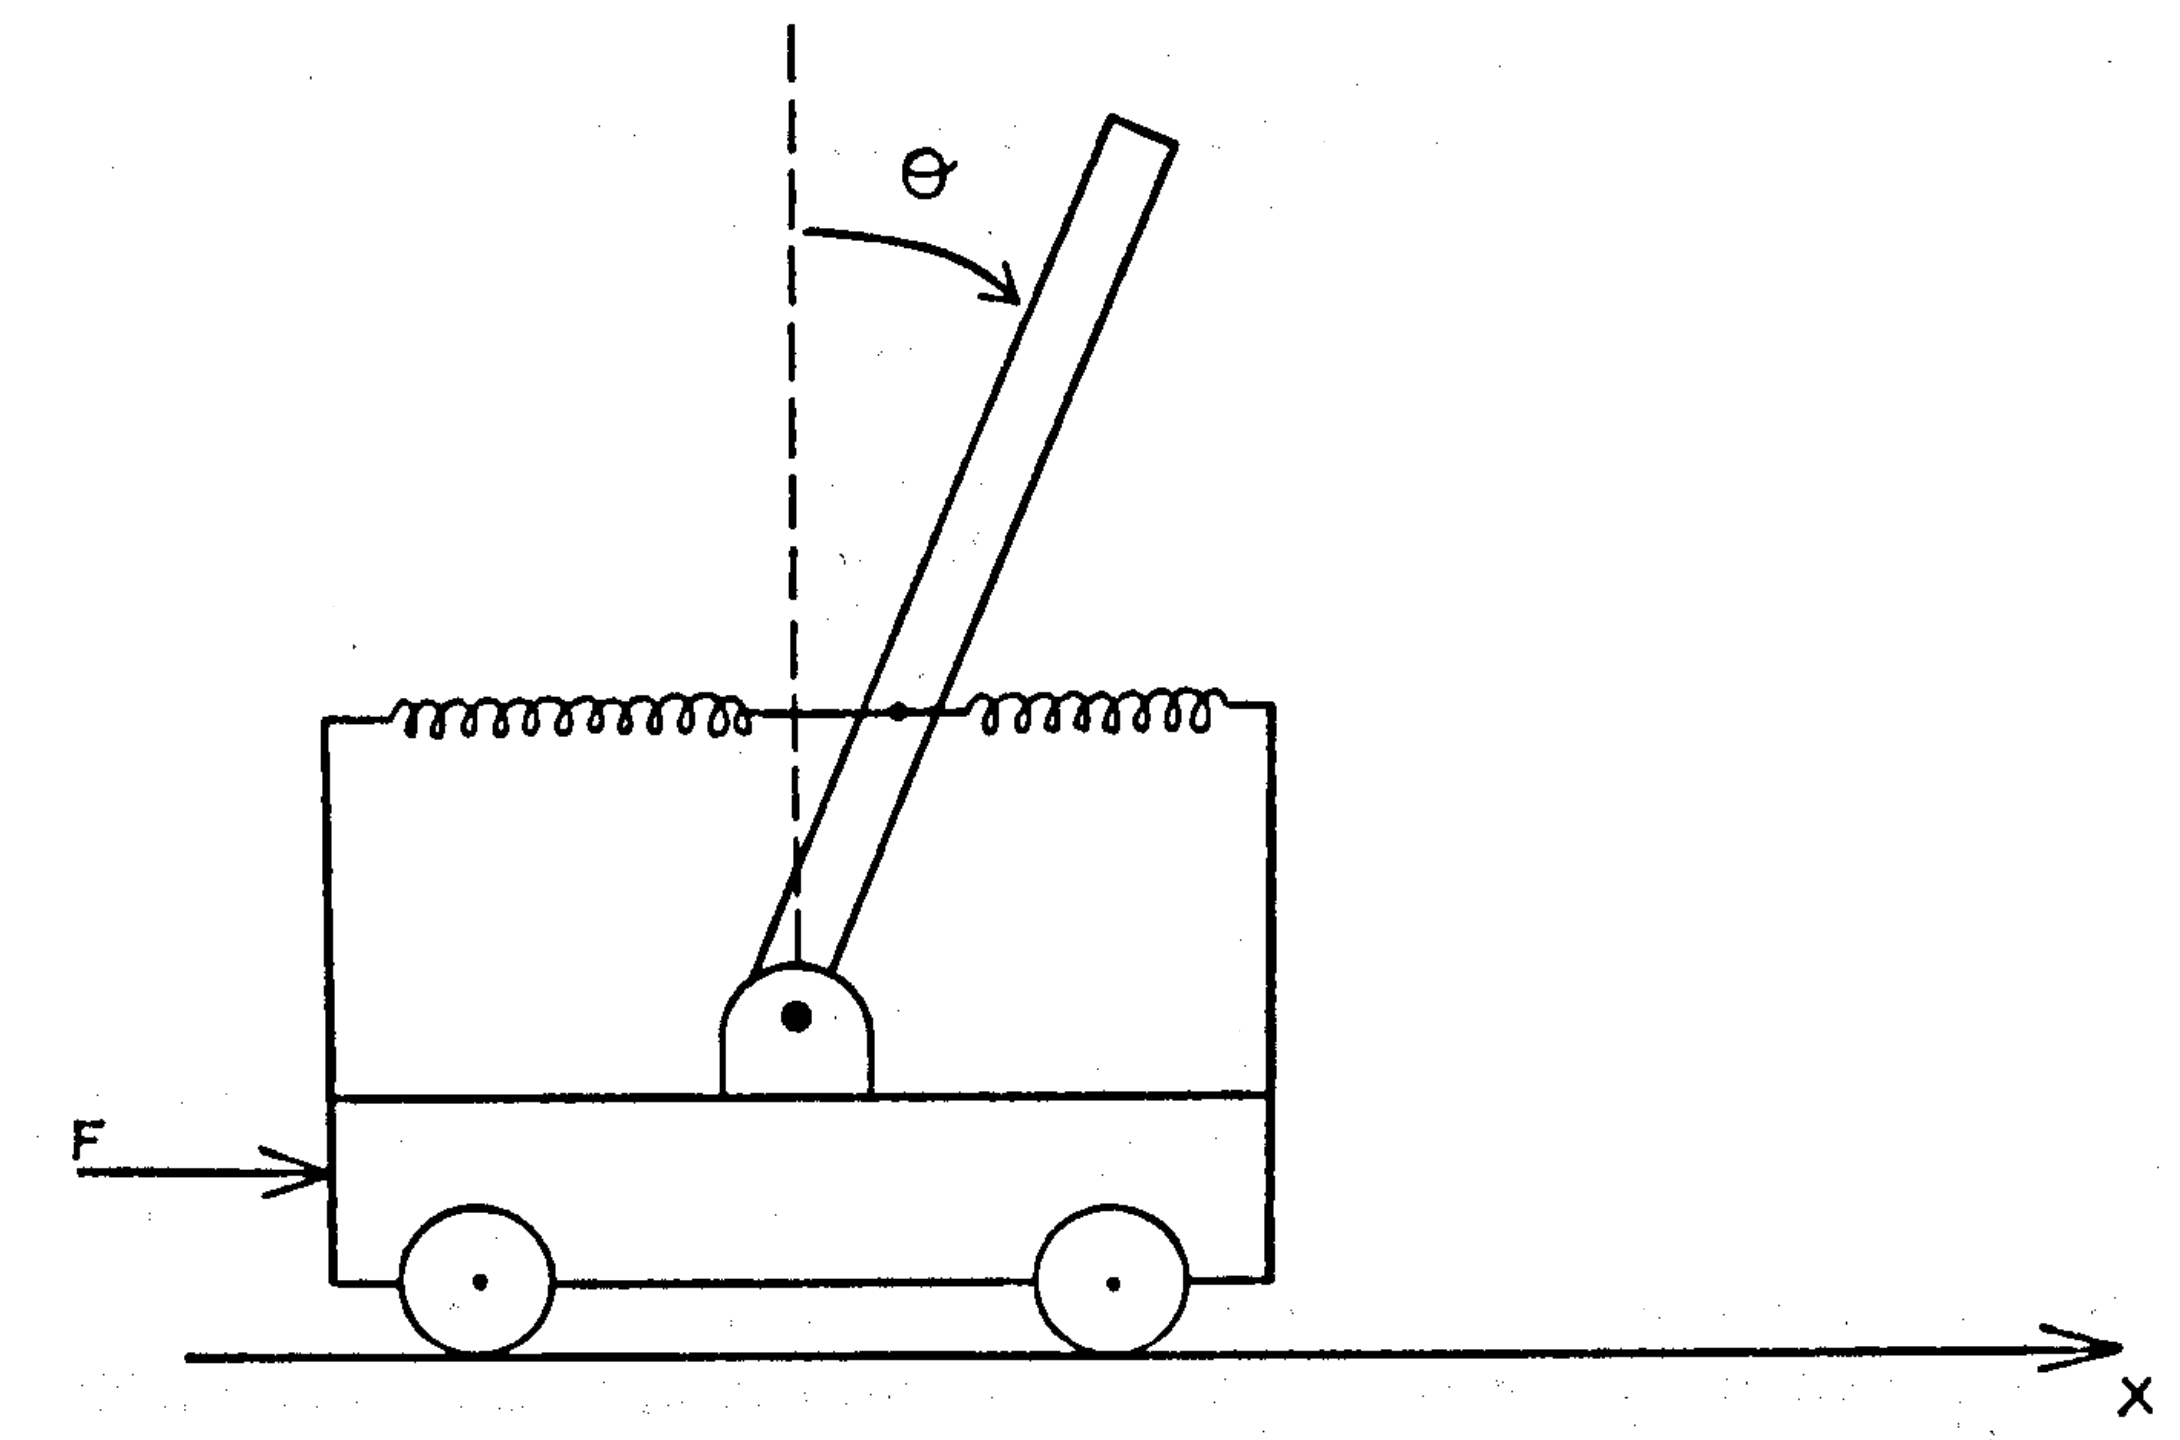
\includegraphics[width=0.7\linewidth]{portada}
	\label{fig:portada}
\end{figure}
	
\thispagestyle{empty}
	
\newpage

\tableofcontents

\newpage
	
	
\section{Introdución}
\subsection{O problema}

Despois de ler e comprender o enunciado da práctica, e de examinar as imaxes unha por unha, chegamos ás seguientes observacións:
\begin{itemize}
	\item Entre as imaxes de barcos existe unha gran variación de pose, escala, condicións de iluminación, proporción que ocupa na escena real (en metros) e proporción que ocupa na imaxen (píxeles). Ademáis os elementos en sí (barcos e peiraos) presentantan moita variación interclase (aínda que os barcos sexan todos industrais son distintos entre eles, e os peiraos poden estar baleiros ou cheos de montañas de area) e incluso unha maior similitude intraclase (sobretodo no caso barco-atracado contra barco-non-atracado).
	\item O alcance da práctica de esta asignatura era suficientemente limitado como para resolver o problema dun xeito satisfactorio. Creemos que poderíamos entrenar unha Rede de Neuronas Artificiais para resolver un subproblema o un problema maior con fin de que a Rede principal o teña máis doado para aprender. No obstante non é o que se pide entón aínda que preferiríamos resolver o problema dunha forma \emph{máis científica} (en vez de simplemente darlle os datos á rede e que ela aprenda) por cuestións de tempo e alcance non o fixemos.
	\item En calqueira escenario (sexa unha práctica con fins docentes ou un traballo no mundo real) existe un problema co cómputo, no noso caso porque disponemos de poucos recursos para adestrar a Rede e no caso real porque o cálculo é posible que precise ser ou a tempo real ou nun sistema embebido, en calqueira caso recursos límitados. 
\end{itemize}

Estas observacións dirixiron o noso \emph{modus operandi}.

\subsection{O noso \emph{modus operandi}}

Aínda que teñamos cursadas asignaturas de aprendizaxe non somos, en nigún caso, expertos no adestramento de Redes de Neuronas Artificiais. Por esta razón preferimos ser cautos e explorar maitas opcións, todas as que podamos, aínda que o noso coñecemento pode (e debería) guiar esta búsqueda, tomamos a decisión de tomar poucas decisións ó principio, e que fora a evidencia a que avale as conclusións. Por esto en vez de faceren unha Red estática, a fixemos altamente flexible. Referímonos a que fixemos un \emph{script} que recibe como argumento unha gran cantidade de hiperparámentros, de xeito que sexa maís cómodo probar. Despóis de algunhas probas (e acompañadas de lecturas da literatura) chegamos ó noso \emph{baseline}.

\section{Clasificación Ship/No-ship}
\subsection{Modelo base}

Describimos agora o noso modelo \emph{baseline}, que valeunos para iterar e comparar resultados. O modelo componse dos seguientes elementos:

\begin{itemize}
	\item  \textbf{EfficientNet.} \cite{tan2019efficientnet} Usámola como CNN (\emph{Convolutional Neural Network}) de partida. Orixinalmente pensamos que tiña como requirimiento que as imaxes sexan de tamaño $(244,244,3)$. E como as imaxes son (i) rectangulares (ii) de distinto tamaño entre sí; tivemos que implementar un recortador automático de \emph{o cadrado máis grande} que chamamos desde os \texttt{DataLoader} de adestramento e proba. Máis tarde decatámosnos que a Rede era realmente capaz de procesar imaxes de calqueira tamaño porque ten ó final un \texttt{Global Pooling}. No obstante, como de calqueira xeito os \emph{mini-batches} tiñan que ser todos del mismo tamaño (paralelepípedos) decidimos quedarnos ca idea de recortalas imaxes da forma mencionada. \\

Máis tarde, non obstante probamos con outros tamaños para o parelelepípedo, coa esperanza de que imaxes rectangulares ofrezcan mellores resultados (en vez de as cadradas) porque estas teñen máis información. Para a nosa sorpresa a evidencia demostrou moito mellor rendimento con imaxes cadradas. Hipotizamos que débese a que como da mesma imaxe rectangular, os cadrados resultantes do resultado aleatorio son realmente distintos entre sí, recortar rectangulos en cadrados pode supor un bo aumento de datos implícito. A continuación pódense ver as curvas de pérdida e precisión de, na esquerda, imaxes rectangulares e, na dereita, imaxes cadradas. Apreciamos que cas imaxes cadradas o adestramento levou máis, foi \emph{máis difícil} pero a cambio xeneraliza moito mellor (a liña discontinua mostra a precisión en proba). (As condicións do adestramento que se mostra foron: sen aumento de datos e sen preentrenado, pero probamos con todas as combinación e a conclusión e consistente.)\\



\begin{figure}[h]
	\centering
	\begin{minipage}{0.45\textwidth}
		\centering
		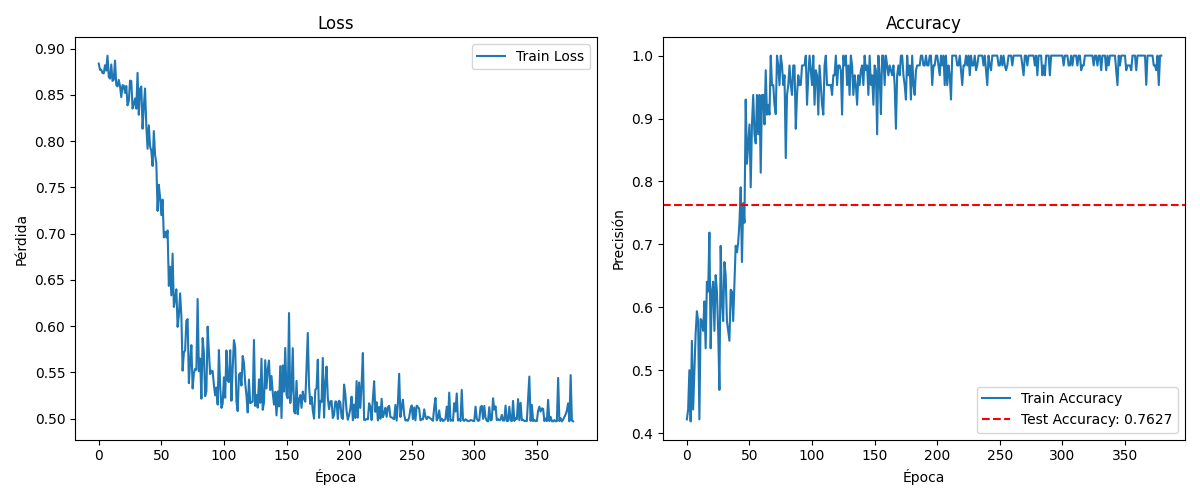
\includegraphics[width=\linewidth]{rectangulo.png}
	\end{minipage}
	\hfill
	\begin{minipage}{0.45\textwidth}
		\centering
		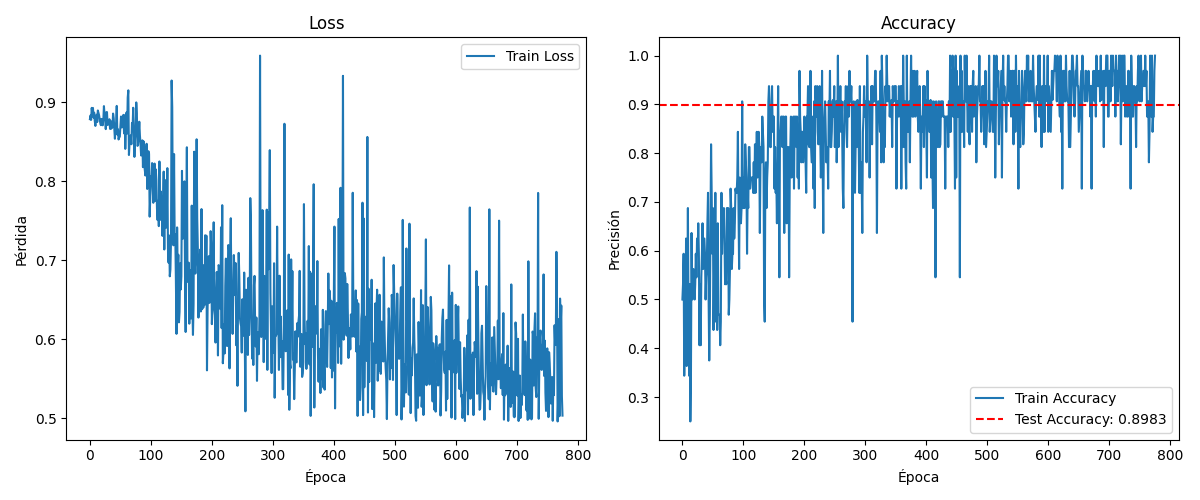
\includegraphics[width=\linewidth]{cadrado.png}
	\end{minipage}
	\label{fig:comparativa}
	\caption{Comparativa de adestramento con imaxes rectangulares (esquerda) e cadradas (dereita)}
\end{figure}






En xeral a motivación para escaller esta rede e non outra débese á terceira observacións da sección 1.1 e á forma que tiveron os autores da Rede de atacar este problema directamente. Con respecto a que EfficientNet en contreto usamos: despóis de probar ca EfficientNetB3 e observar malos resultados decidimos mudar á EfficientNetB4 e nos quedamos nesta e non subimos á EfficientNetB$i \; |\; i\; \in \{5,6,7\}$ precisamente por limitacións de cómputo.

	\item \textbf{Aumento de datos.} O aumento de datos nesta fase esencialmente consta de dúas partes, por un lado, as transformacións de \texttt{torchvision.transforms} e por otro imaxes recortadas a man. Con respecto ó  primeiro, nosotros usamos: volteos horizontais, fluctuacións leves na cor, tamén leves transformacións afíns, conversión a blanco e negro e emborronado Gausiano. O segundo punto é que recortamos manualmente as imaxes de barcos de forma que queden centrados e sen fondo que estorbe, engadíronse estas imaxes ó conxunto de datos cando especificabase aumento de datos e clasificación en dúas clases (non consideramos adecuado incluir estas imaxes na clasificación de tres clases porque ahí é importante o contexto do barco). As transformacións pódense apreciar na figura \ref{fig:aumento}. Desta forma conseguimos dúas cousas distintas: 
	\begin{itemize}
		\item Representar máis variacións das presentes no conxunto de adestramento, ca esperanza de que se sí ocurriesen no conxunto de proba, estaríamos preparados. Por exemplo, como observamos imaxes de noite ou con chuvia encontramos razonable incluir a conversión a blanco e negro.
		\item Representar con menos ruído adicional o que sí queremos aprender. Porque aínda que é beneficioso para a Rede someterse a moita variación, tamén dificulta o adestramento (é un problema máis difícil).
\end{itemize}

\begin{figure}[h]
	\centering
	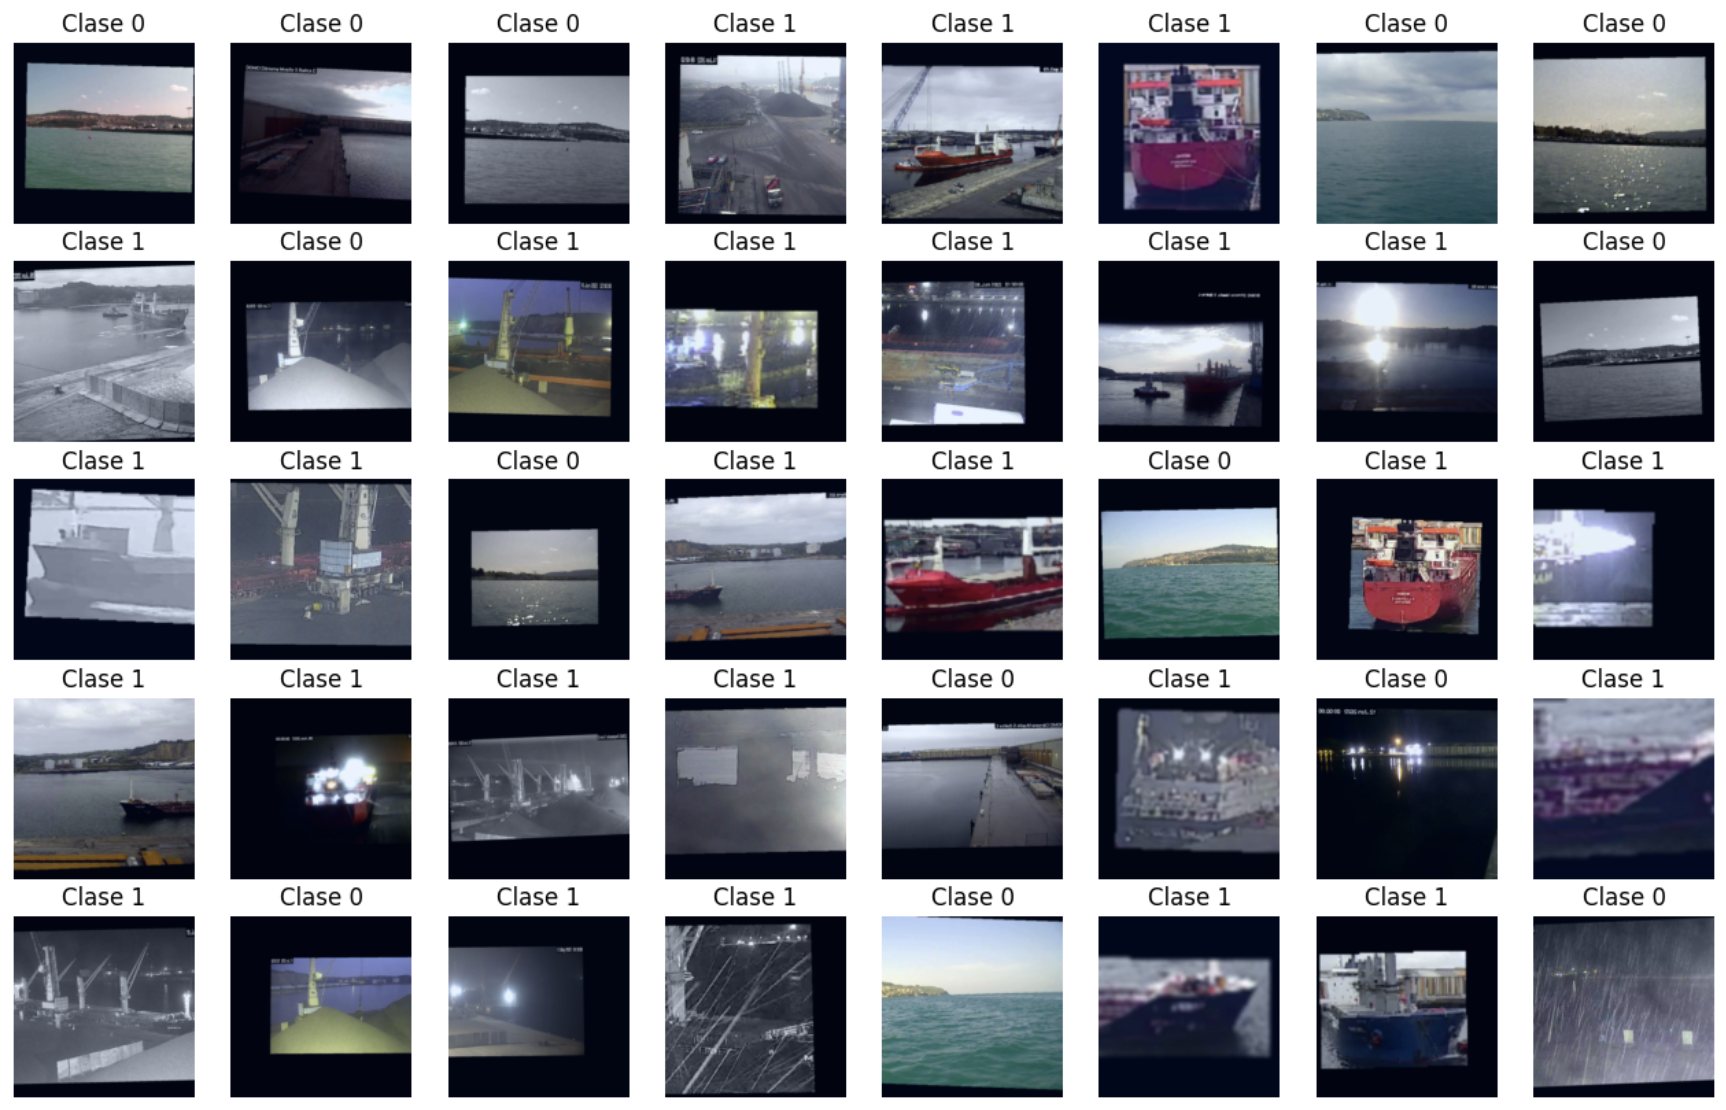
\includegraphics[width=0.9\linewidth]{aumentoDatosEx1.png}
	\caption{Imaxes cas transformacións do aumento de datos}
	\label{fig:aumento}
\end{figure}

Sobre o aumento de datos comentar que a relación dos hiperparámetros que o definen e problemática para nos faceren probas: se cambiamos varios de unha vez non está necesariamente claro a cal dos cambiados débese a mellora ou empeora do rendimiento; se, en cambio, cambiamos só un de cada vez, a búsqueda no espacio de hiperparámetros do aumento de datos vólvese prohibitiva. E por isto que sabemos que a nosa configuración debe ser subóptima, pero non temos nada para evitalo.
\item Un \textbf{MLP} (Perceptrón Multicapa ou \emph{Multi-layer Perceptron} en ingés) de tres capas, sobre a saída da Rede. A saída da última capa \texttt{nn.Softmax()} ten 2 o 3 neuronas según se quería clasificar en \{no barco, barco\} o en \{no barco, barco no amarrado, barco amarrado\}. Tamén probamos con un perceptrón simple (unha capa) pero a evidencia demostrou que os resultados eran mellores con tres. Como o número de neuronas na primeira capa (a saída da CNN) era máis grande ca o número de exemplos, a rede podería ter aprendido unha solución trivial co conxunto de adestramento e non xeneralizar en absoluto. Por esto mismo decantamos por usar a ben coñecida técnica de regularización \emph{DropOut} \cite{srivastava2014dropout}. 
\end{itemize}

\subsection{Adestramento e evaluación}

O adestramento foi díficil e ademáis somos inexpertos porén indentificamos algúns problemas para os que atopamos solución. Aquí preséntanse:
\begin{itemize}
	\item \textbf{Datos non balanceados.} Observamos que a Rede, \emph{hackeando} as nosas métricas decidía que todas as imaxes eran barcos. Esto débese ó desbalanceo dos datos (147 contra 88) dónde unha solución tan trivial e erronea como solo predecir unha clase non estaba tan penalizado con metricas como a precisión. Afrontamos isto alterando a probabilidade de ocurrencia das clases de forma que se antes, ó escolleren unha imaxe de \texttt{DataLoader}, $p(X=barco) = \frac{147}{147+88}$ ahora $p(X = barco) = 0.5$. Para ello usamos a utilidad \texttt{WeightedRandomSampler} de torch.
	\item \textbf{Similitud nos datos.} Non creemos conveniente que a Rede esté totalmente segura de que un barco non está (porque igual é pequeno ou está ocluído) cando ela dí que non hai barco na imaxe. Por isto, e para que xeneralice millor adoptamos a idea de \cite{DBLP:journals/corr/SzegedyVISW15} donde as etiquetas en vez de ser [0, 1] para non-barco e [1, 0] para barco, son [$\epsilon$,$1 - \epsilon$] e [$1- \epsilon$,$\epsilon$] respectivamente, onde fixamos $\epsilon = 0.1$.
	\item \textbf{Capacidade do modelo.} Orixinalmente usamos a EfficientNetB0, pero apreciando malos resultados decidimos mudar á EfficientNetB3 e logo á EfficientNetB4, que é un pouco máis grande pero precisamente como narran no artículo, é eficiente. Probamos con outras alternativas como as clásicas ResNet e VGGNet sen conseguiren melloras nos resultados que pagasen a pena a diferencia no consumo de recursos.
	\item \textbf{Mínimos locais.} Para aliviar as consecuencias da dificultade do adestramento implementamos un \texttt{learning\_rate} que, con unha certa paciencia, mediaba a sua valor. \footnote{Esta paciencia mencionada e a do \emph{earlystopping} poden ambas ser axustadas como \emph{flags} no noso \emph{script}.}
	\item \textbf{Sobreajuste e xeneralización.} Para cercionarnos de que a Rede aprendía correctamente, añadimos una penalización de la norma euclídea dos parámetros na función de perdida, es decir, regularización Tikhonov. Atopar valores axeitados para $\lambda$ foi especialmente difícil.
\end{itemize}


\begin{wrapfigure}[10]{l}{0.35\textwidth}
	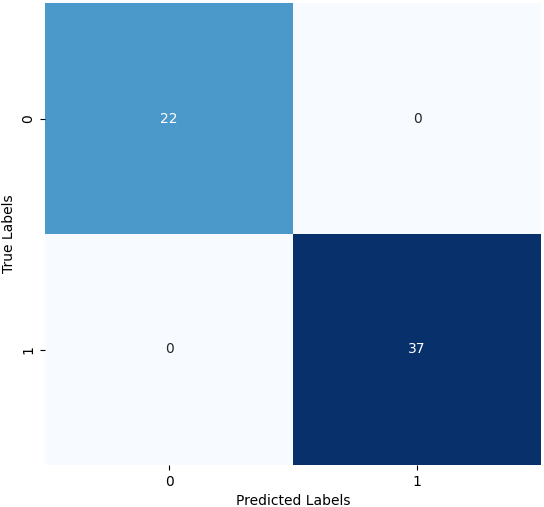
\includegraphics[width=1\linewidth]{cmEj1} 
	\label{fig:cmEj1}
	%\caption{Matriz de confusión para el primer ejercicio}
\end{wrapfigure}


Outras consideracións sobre o adestramento que consideramos menos profundas e más ordinarias son: como optimizador usamos AdamW \cite{DBLP:journals/corr/abs-1711-05101} con un \texttt{learning\_rate} de $10^{-3}$ ou $10^{-4}$. Usamos un \texttt{batch\_size} de 32.

Con respecto ós resultados obtidos nesta primeira iteración, poden observarse a grandes rasgos na matriz de confusión da esquerda. Figuras das curvas de pérdida e precisión en aprendizaxe ou das etiquetas predichas pola Rede para algunhas imágenes en concreto poden atoparse para este exercicio e o seguiente no Apéndice ó final del documento. \\
\\
\newpage 
\section{Clasificación Docked/Undocked}

Nós concebimos este exercicio como unha extensión do anterior, deste xeito pensamos en reutilizar todas as representacións aprendidas.
\begin{itemize}
	\item Cuando especifícase \texttt{pretrained=True}, a nosa Rede non toma os parámetros de Imagenet, senon do exercicio anterior. Deste xeito xa ten moito aprendido e o proceso de optimización será más doado.
	\item Como agora a cabeza da Rede ten 3 neuronas pero antes tiña 2, en vez de inicializar aleatoriamente las tres neuronas, dous copianse e só unha inicializase aleatoriamente. De novo, deste xeito ten menos traballo por diante. De calqueira xeito esperaríamos que a rede mude moito os seus parámetros durante o adestramento e esta inicialización soamente é unha inicialización aforturanda, pero por suposto é preciso adestrar a Rede (con moitas épocas).

\end{itemize}


\begin{wrapfigure}[14]{l}{0.35\textwidth}
	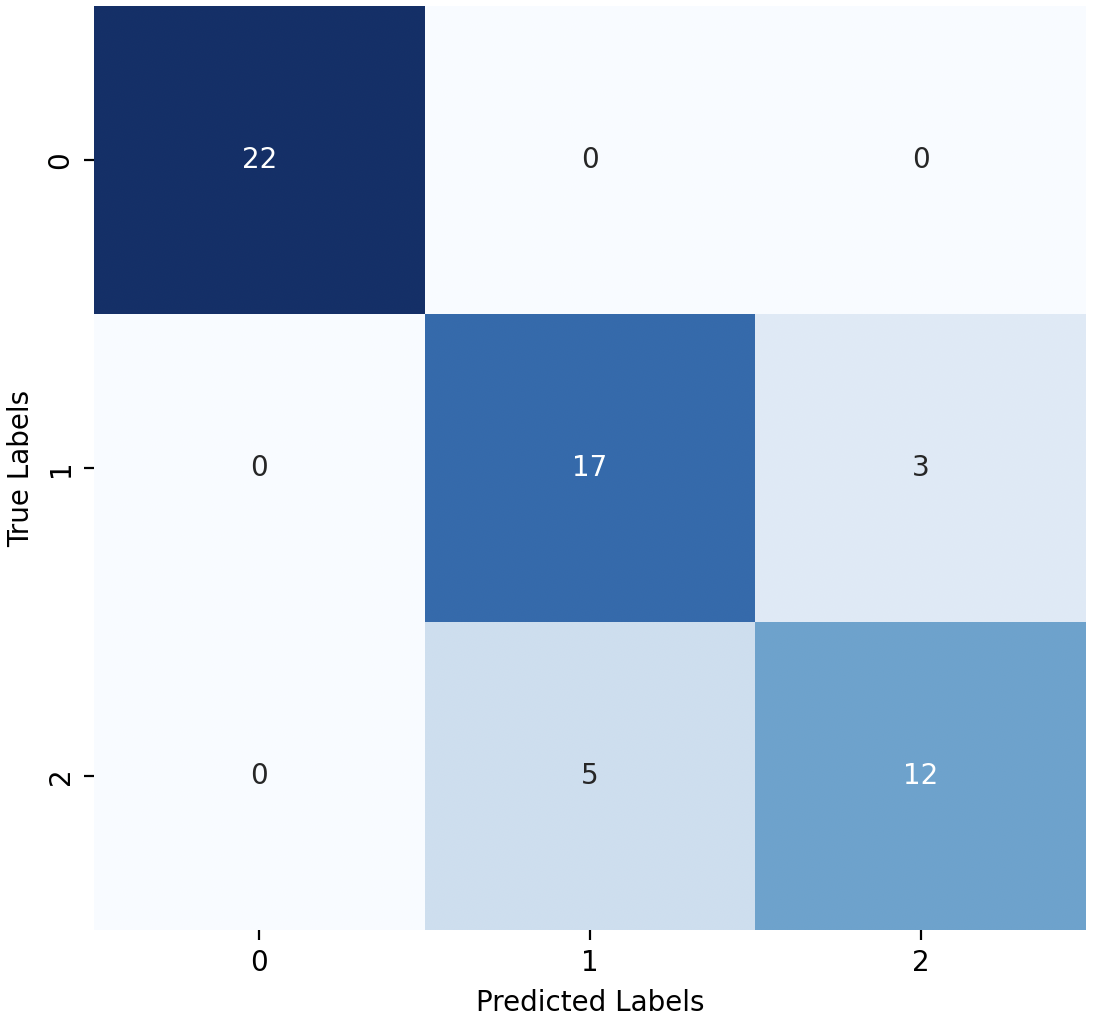
\includegraphics[width=1\linewidth]{cmEj2} 
	\label{fig:cmEj2}
	%\caption{Matriz de confusión para el segundo ejercicio}
\end{wrapfigure}

Ainda que a priori semella que son peores resultados que no exercicio 1, queremos sinalar as seguintes observacións:

\begin{itemize}
	\item Agora o problema orixinal (barco contra no barco) está totalmente resolto (no barco tiene la etiqueta de 0). A isto encontramoslle a seguiente intuición: que a Rede se esforce nun problema máis complexo fai que sexa máis capaz de resolver o problema sinxelo.
	\item As diferenzas entre as clases atracado contra no atracado son realmente sutiles (ver Figura \ref{fig:comparativaDoked}) e a un humano (nós probamos con amigos) que non foi \emph{adestrado} cas etiquetas tamén pode resultarlle complexo resolver. 
	\item Non obstante en xeneral poderíamos dicir que malia non seren a clasificación perfecta, polo  menos é bastante diagonal.
\end{itemize}


\begin{figure}[h]
	\centering
	\begin{minipage}{0.45\textwidth}
		\centering
		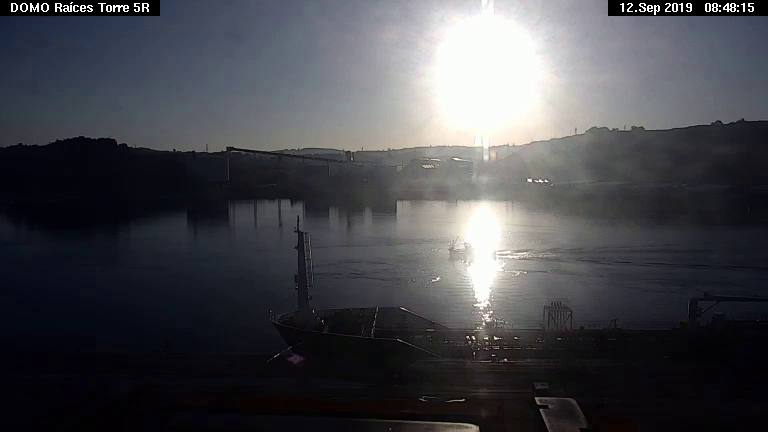
\includegraphics[width=\linewidth]{docked.jpg}
	\end{minipage}
	\hfill
	\begin{minipage}{0.45\textwidth}
		\centering
		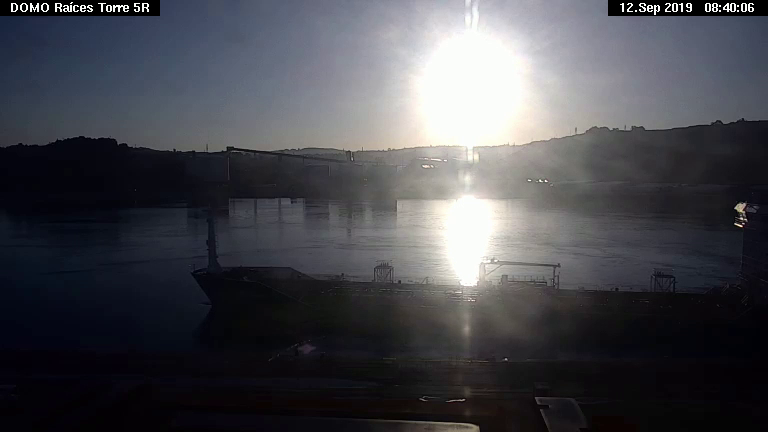
\includegraphics[width=\linewidth]{undocked.jpg}
	\end{minipage}
	\label{fig:comparativaDoked}
	\caption{Comparativa dunha imaxen do barco amarrado (esquerda) e no mar (dereita)}
\end{figure}

\newpage
\section{Evaluación dos modelos}

Na tabla a continuación mostránse os resultados da precisión das prediccións da Rede cos datos de proba, a separación de datos adestramento e proba foi dun 80\%

\begin{table}[H]
\begin{tabular}{l|cc|cc|}
\cline{2-5}
                               & \multicolumn{2}{c|}{Non preentrenado}                        & \multicolumn{2}{c|}{Preentrenado}                            \\ \cline{2-5} 
                               & \multicolumn{1}{c|}{Non aumento de datos} & Aumento de datos & \multicolumn{1}{c|}{Non aumento de datos} & Aumento de datos \\ \hline
\multicolumn{1}{|l|}{2 clases} & \multicolumn{1}{c|}{94\%}                 & 84\%             & \multicolumn{1}{c|}{100\%}                & 98\%             \\ \hline
\multicolumn{1}{|l|}{3 clases} & \multicolumn{1}{c|}{76\%}                 & 67\%             & \multicolumn{1}{c|}{86\%}                 & 83\%             \\ \hline
\end{tabular}
\end{table}

Sobre estos resultados podense facer as seguintes reflexións:
\begin{itemize}
	\item Que o modelo esté preentrenado ou non supón unha gran diferencia, sobretodo no caso de aumento de datos. Esto é loxico e esperable. Que ocurra máis claramente no caso de aumento de datos xustificase con que: ó seren un problema máis difícil, vai ser maior a axuda que supón ter os parámetros preentrenados.
	\item O aumento de datos sempre ofrece peores resultados que non facelo. Esto pode parecer alarmante, e indicador de que fixemos un mal aumento de datos. Pero hai varias cousas que matizar. En primer lugar, como en calqueira caso as imaxes rectangulares recortanse a cadrados, sempre hai algún timpo de aumento de datos, entón na táboa realmente estase a mostrar a comparativa de aumento de datos ou moito aumento de datos. Ademáis é posible que con máis épocas a Rede seguise adestrándose ata o punto de que con aumento de datos exista unha mellora. Ó final o obxectivo do aumento de datos e impoñer restriccións sobre o que debe aprender ca esperanza de que xeneralice mellor; por tanto, ó enfrentar á Rede a un problema maior, que lle custe máis é esperable.
	\item En calqueira caso vemos que no problema de clasificación en dúas clases non fai falla aumento de datos.
\end{itemize}


\section{Conclusión}

Agradecemos que o conxunto de datos desta práctica fora realista porque intentando obter mellores resultados tivemos que probar e aprender moitas cousas. Creemos, non obstante, que se tivesemos que resolver este problema nun contexto real, debería intentarse algunha aproximación más centrada en visión e non tan \emph{darlle os datos á rede e que ela aprenda}. Ou incluso usar arquitecturas máis sofisticadas que intenten resolver un problema más complexo como segmentación coa esperanza de que o rendimento na tarea más sinxela de clasificación véxase mellorado.

\newpage

\section{Apéndice A: figuras}
\subsection{Primeiro exercicio}
\subsubsection{Sen Aumento de datos e sen Preentrenado}
\begin{figure}[H]
    \centering
    \begin{minipage}{0.55\textwidth}
        \centering
        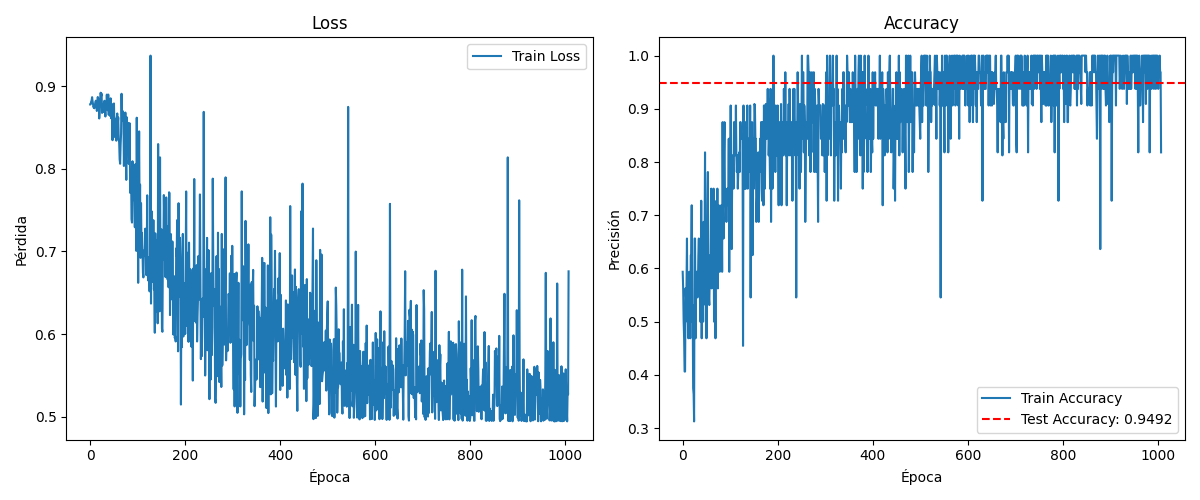
\includegraphics[width=\linewidth]{../ultimas_figuras/LOSS__A_False_P_False_D_False_MLP_True_efficientnet_b4.png}
    \end{minipage}
    \begin{minipage}{0.3\textwidth}
        \centering
        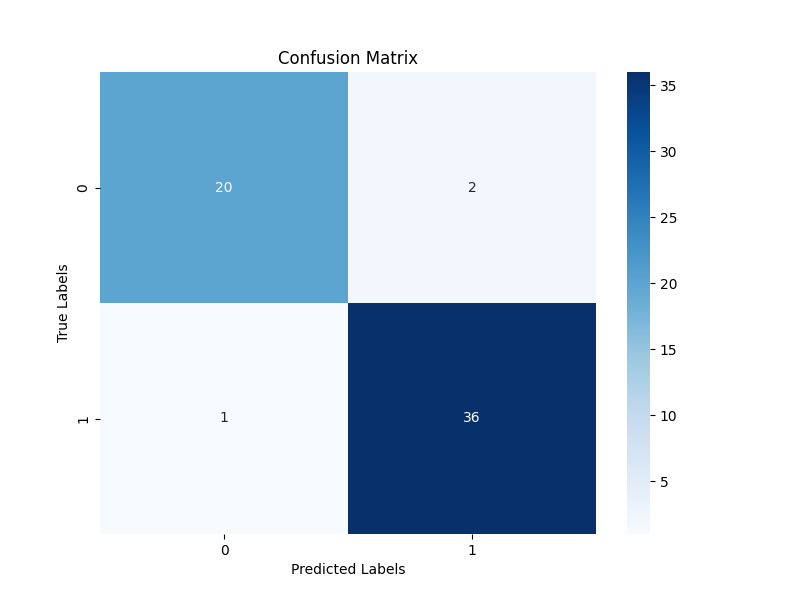
\includegraphics[width=\linewidth]{../ultimas_figuras/CM__A_False_P_False_D_False_MLP_True_efficientnet_b4.png}
    \end{minipage}
    \begin{minipage}{0.7\textwidth}
        \centering
        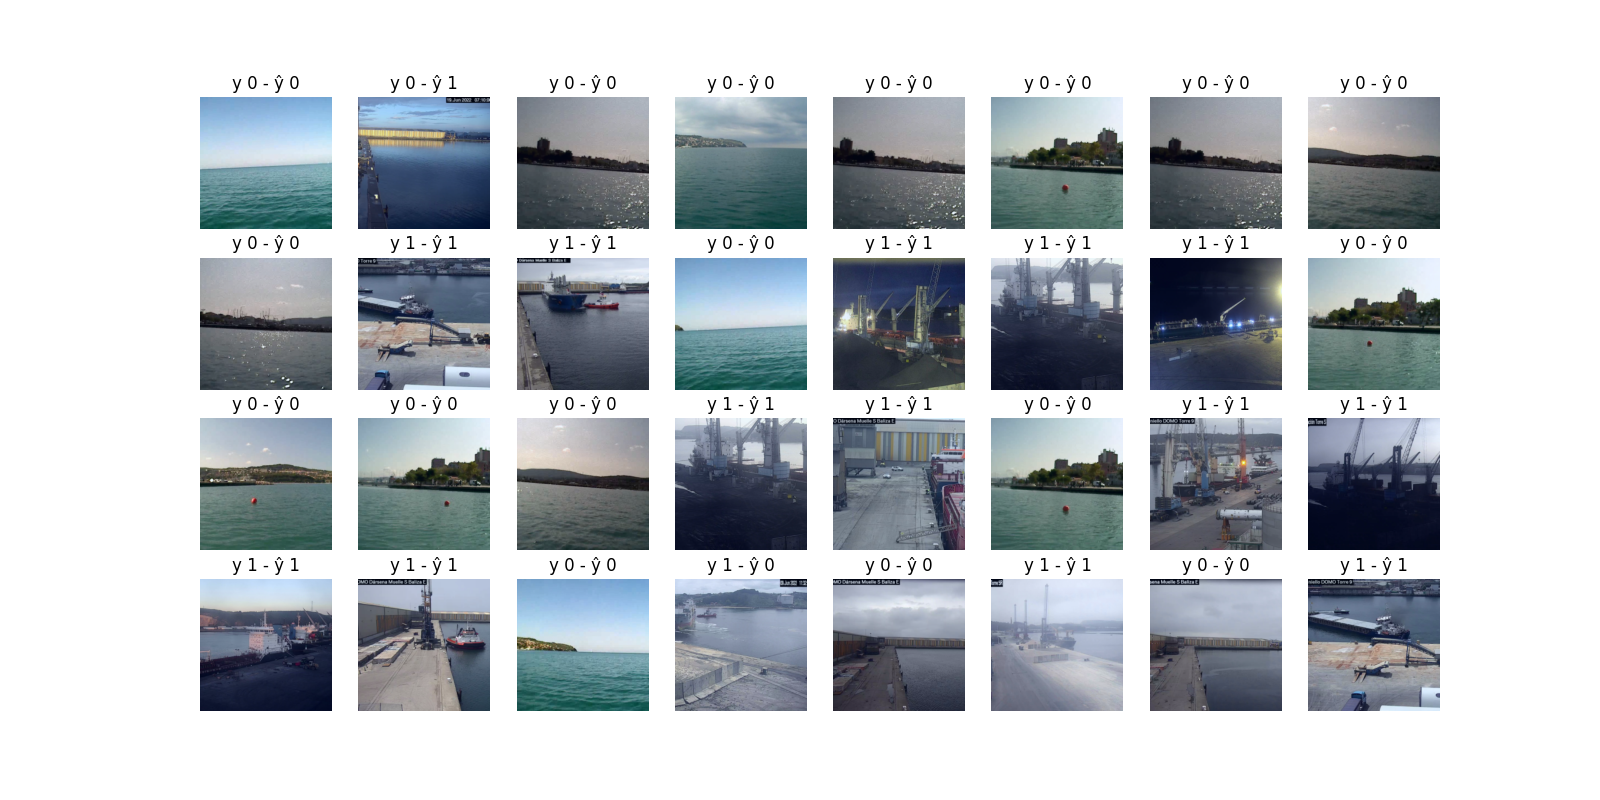
\includegraphics[width=\linewidth]{../ultimas_figuras/GRID__A_False_P_False_D_False_MLP_True_efficientnet_b4.png}
    \end{minipage}
\end{figure}
\subsubsection{Sen Aumento de datos e con Preentrenado}
\begin{figure}[H]
    \centering
    \begin{minipage}{0.55\textwidth}
        \centering
        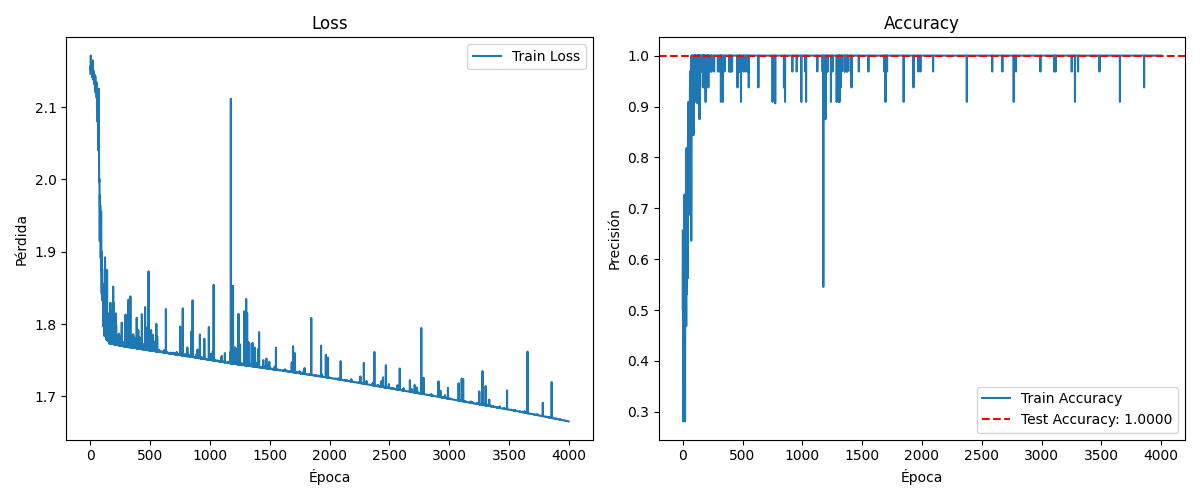
\includegraphics[width=\linewidth]{../ultimas_figuras/LOSS__A_False_P_True_D_False_MLP_True_efficientnet_b4.png}
    \end{minipage}
    \begin{minipage}{0.3\textwidth}
        \centering
        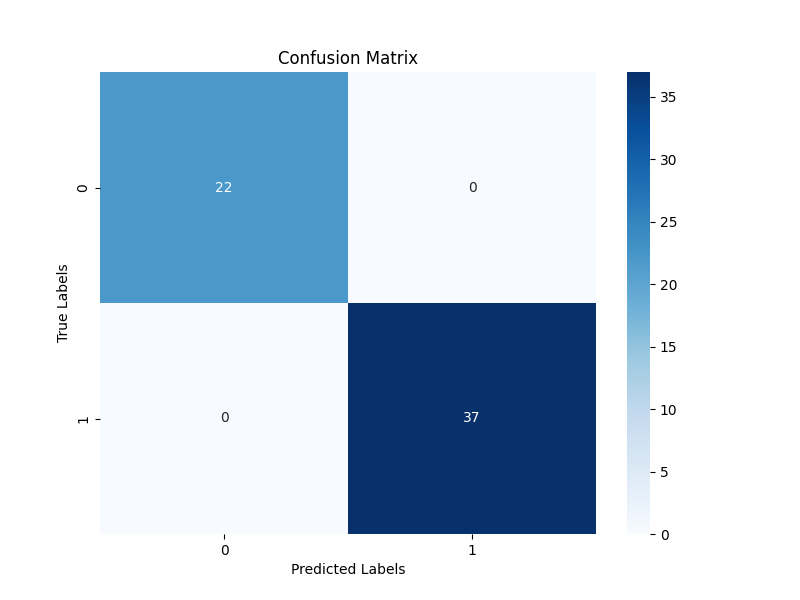
\includegraphics[width=\linewidth]{../ultimas_figuras/CM__A_False_P_True_D_False_MLP_True_efficientnet_b4.png}
    \end{minipage}
    \begin{minipage}{0.7\textwidth}
        \centering
        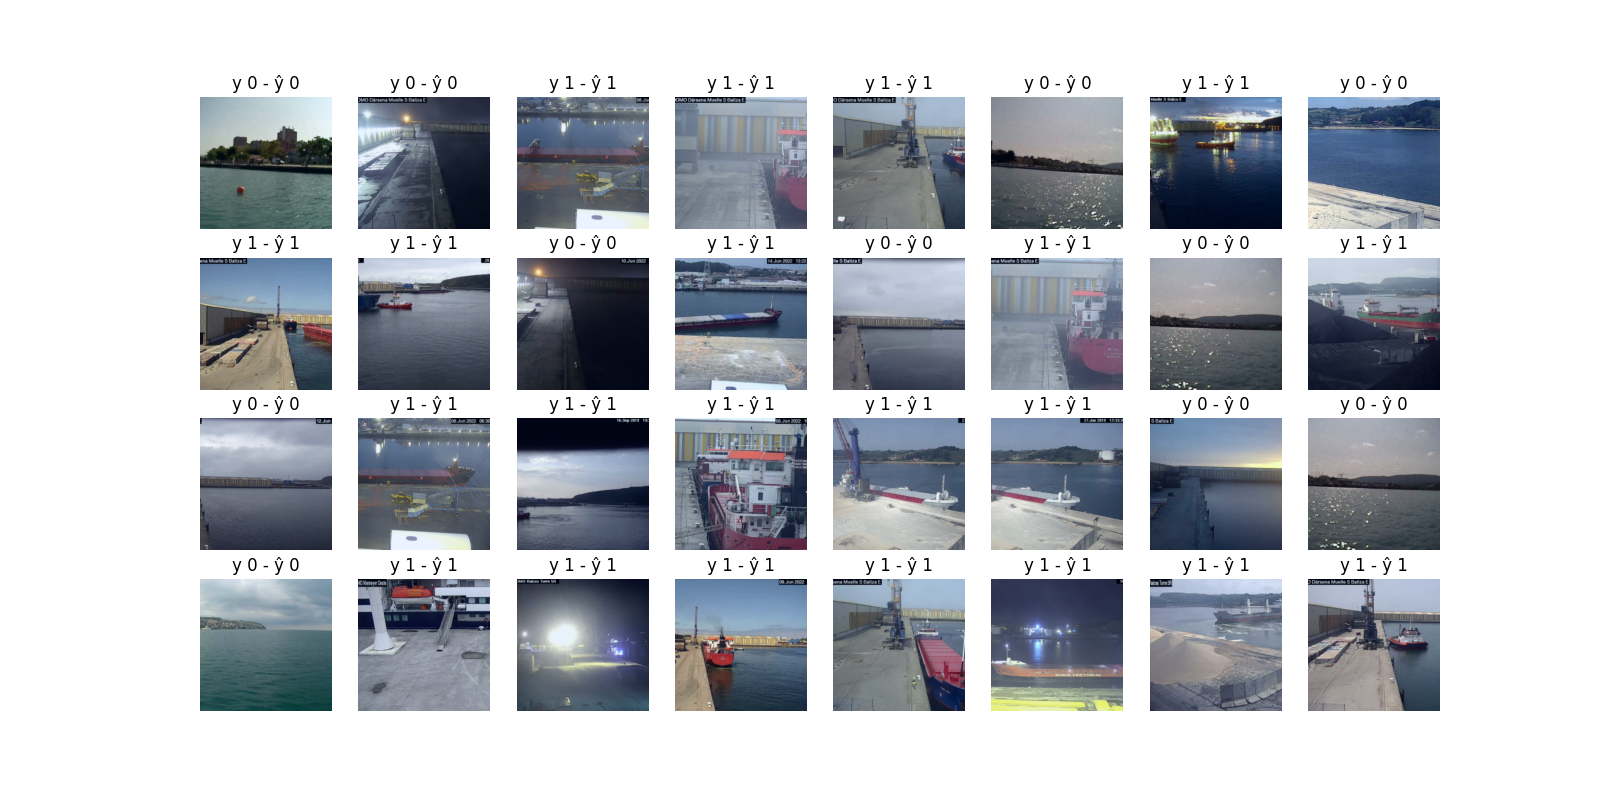
\includegraphics[width=\linewidth]{../ultimas_figuras/GRID__A_False_P_True_D_False_MLP_True_efficientnet_b4.png}
    \end{minipage}
\end{figure}
\subsubsection{Con Aumento de datos e sen Preentrenado}
\begin{figure}[H]
    \centering
    \begin{minipage}{0.55\textwidth}
        \centering
        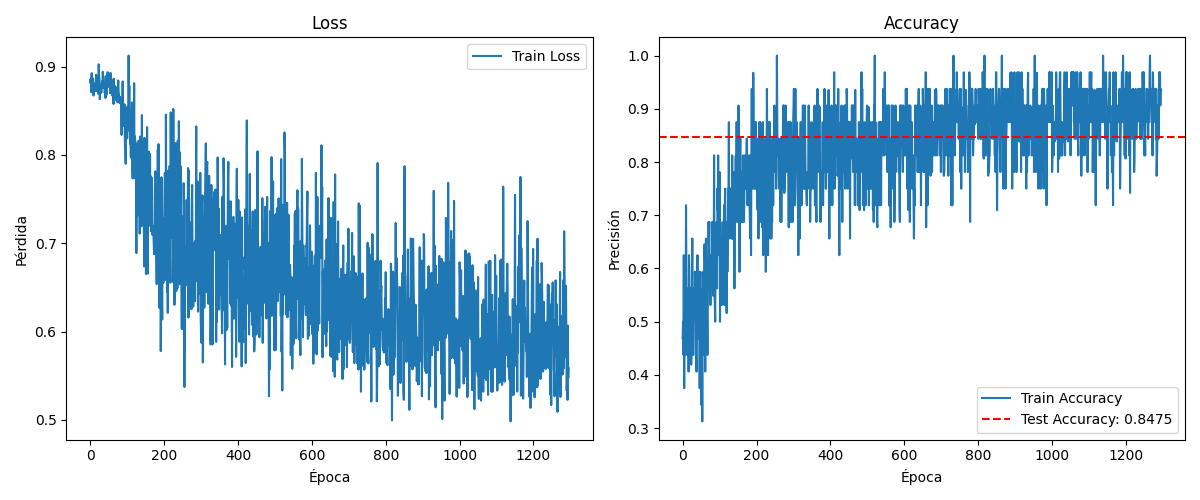
\includegraphics[width=\linewidth]{../ultimas_figuras/LOSS__A_True_P_False_D_False_MLP_True_efficientnet_b4.png}
    \end{minipage}
    \begin{minipage}{0.3\textwidth}
        \centering
        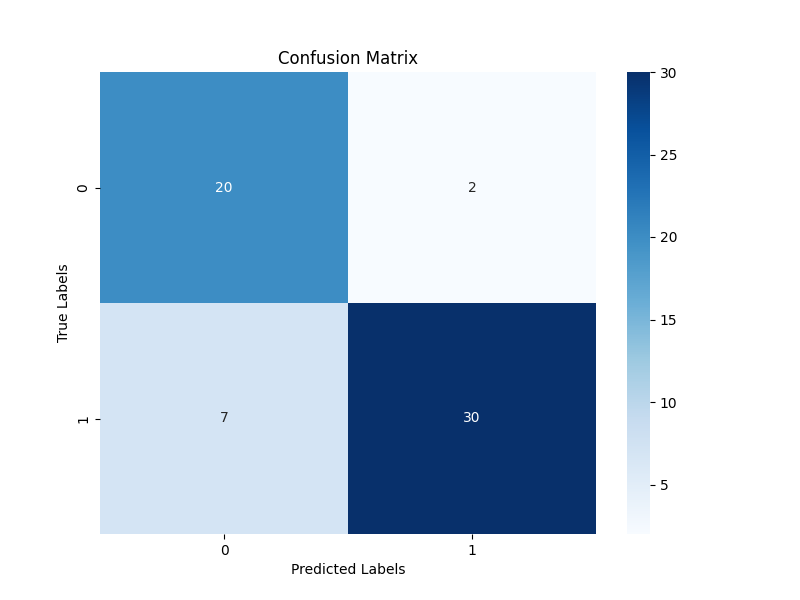
\includegraphics[width=\linewidth]{../ultimas_figuras/CM__A_True_P_False_D_False_MLP_True_efficientnet_b4.png}
    \end{minipage}
    \begin{minipage}{0.7\textwidth}
        \centering
        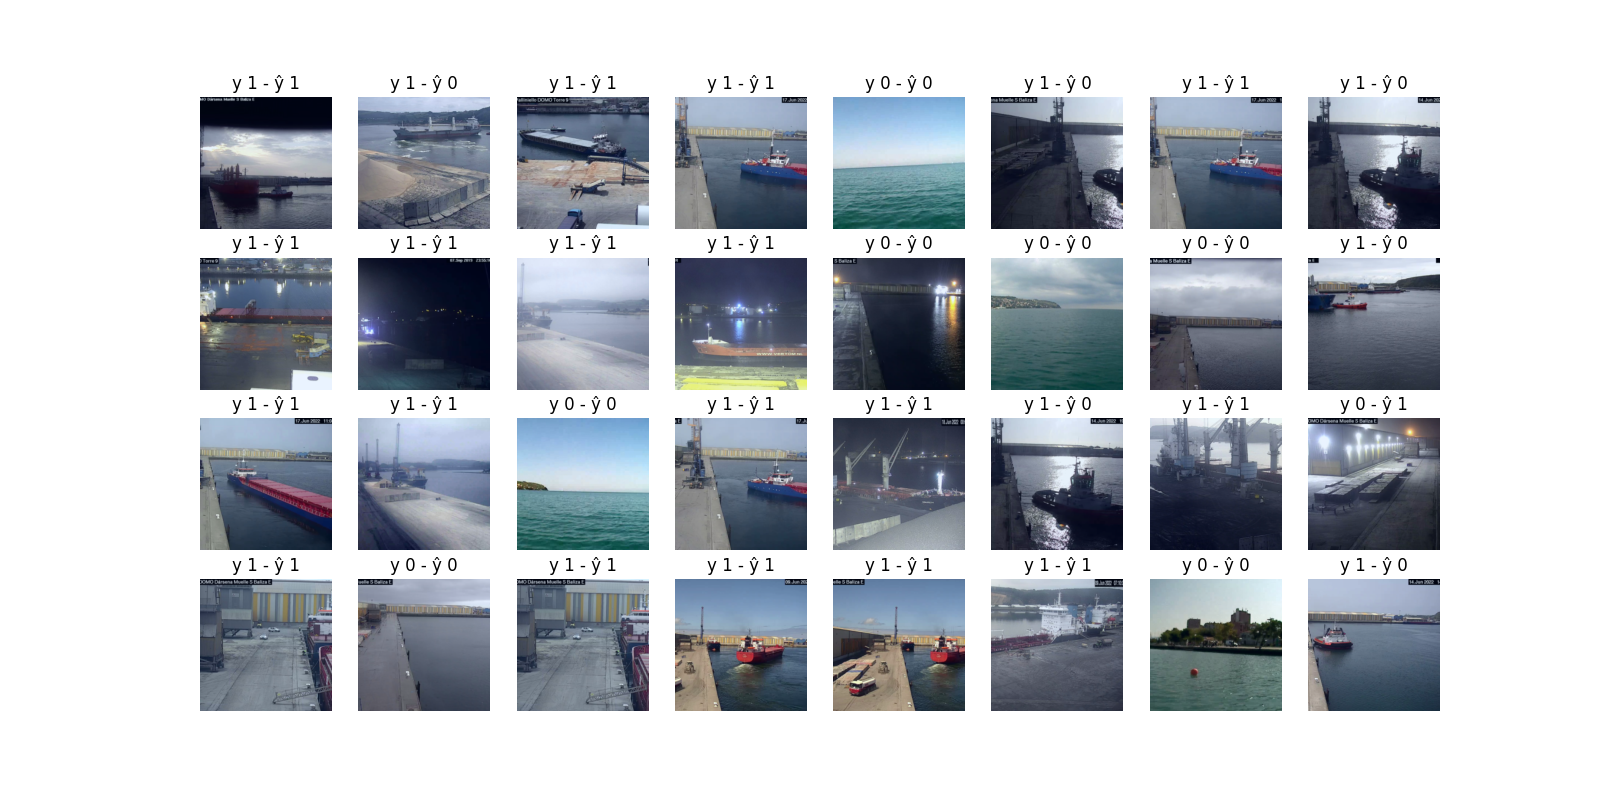
\includegraphics[width=\linewidth]{../ultimas_figuras/GRID__A_True_P_False_D_False_MLP_True_efficientnet_b4.png}
    \end{minipage}
\end{figure}
\subsubsection{Con Aumento de datos e con Preentrenado}
\begin{figure}[H]
    \centering
    \begin{minipage}{0.55\textwidth}
        \centering
        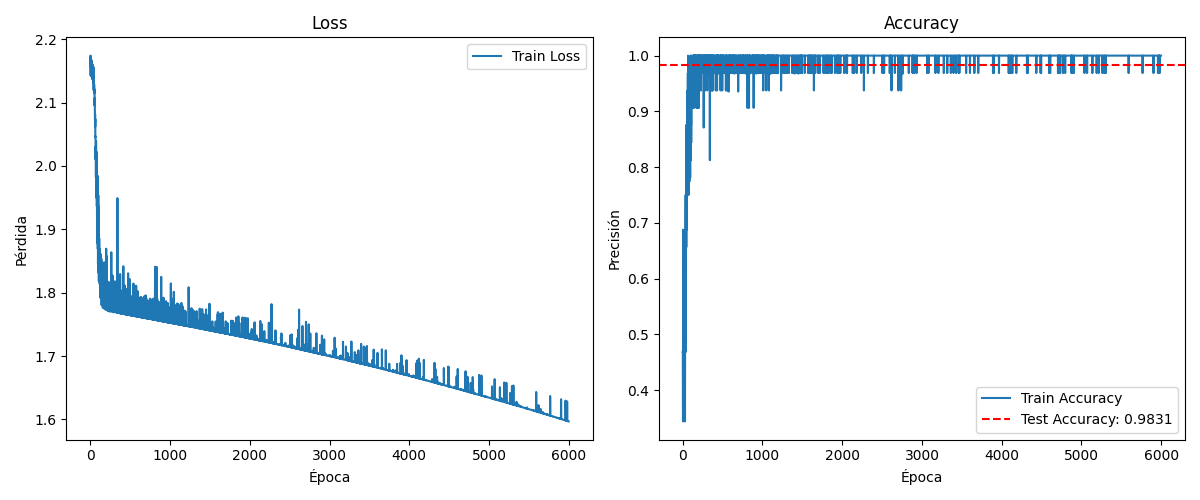
\includegraphics[width=\linewidth]{../ultimas_figuras/LOSS__A_True_P_True_D_False_MLP_True_efficientnet_b4.png}
    \end{minipage}
    \begin{minipage}{0.3\textwidth}
        \centering
        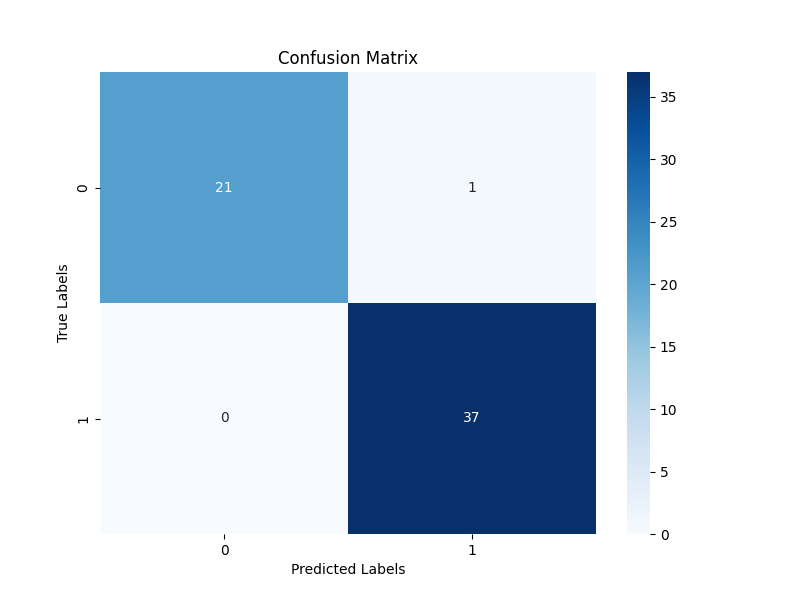
\includegraphics[width=\linewidth]{../ultimas_figuras/CM__A_True_P_True_D_False_MLP_True_efficientnet_b4.png}
    \end{minipage}
    \begin{minipage}{0.7\textwidth}
        \centering
        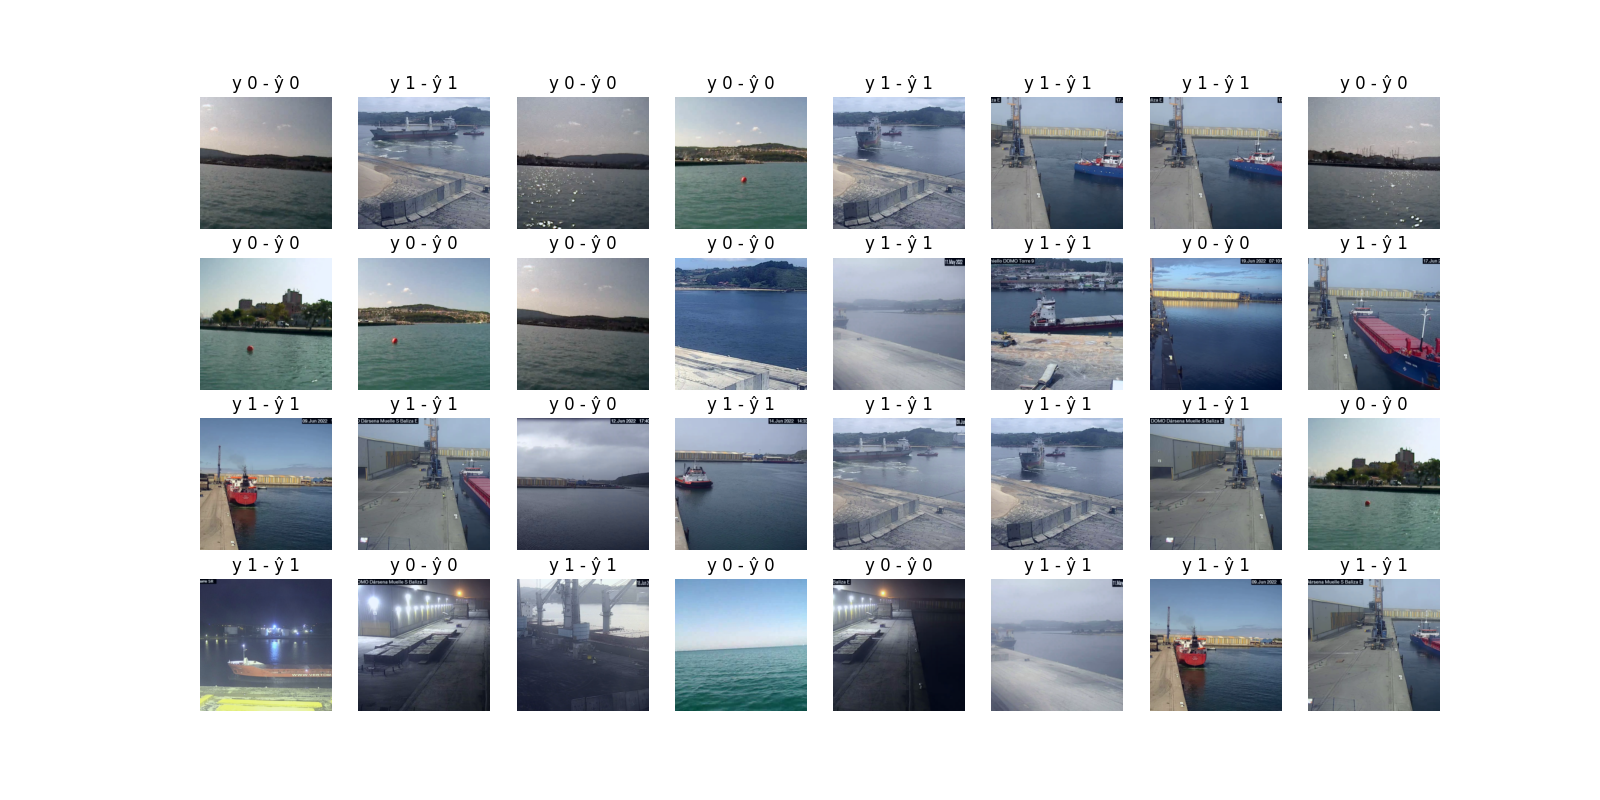
\includegraphics[width=\linewidth]{../ultimas_figuras/GRID__A_True_P_True_D_False_MLP_True_efficientnet_b4.png}
    \end{minipage}
\end{figure}
\subsection{Segundo exercicio}
\subsubsection{Sen Aumento de datos e sen Preentrenado}
\begin{figure}[H]
    \centering
    \begin{minipage}{0.55\textwidth}
        \centering
        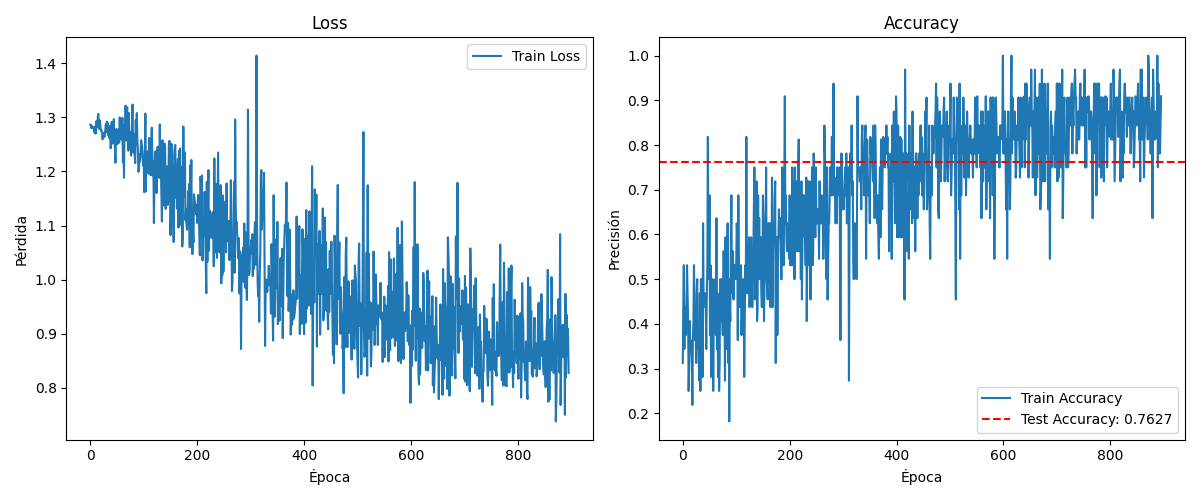
\includegraphics[width=\linewidth]{../ultimas_figuras/LOSS__A_False_P_False_D_True_MLP_True_efficientnet_b4.png}
    \end{minipage}
    \begin{minipage}{0.3\textwidth}
        \centering
        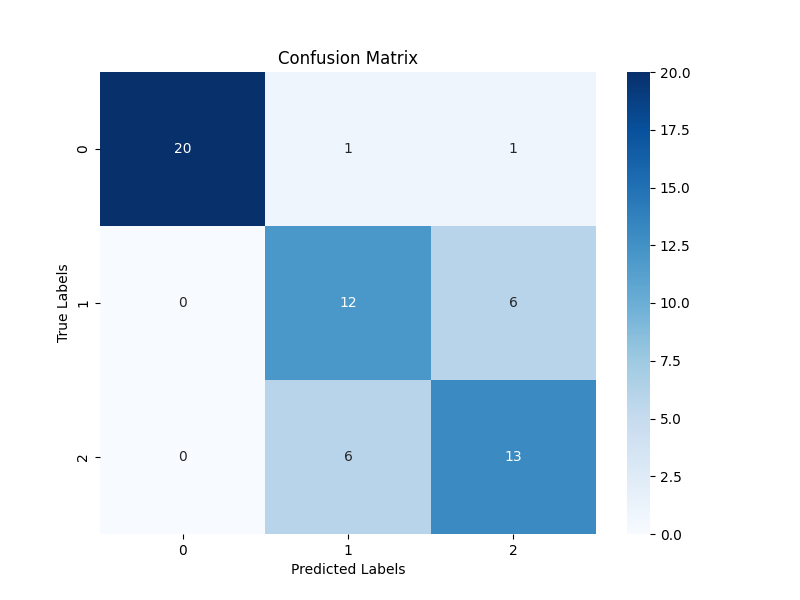
\includegraphics[width=\linewidth]{../ultimas_figuras/CM__A_False_P_False_D_True_MLP_True_efficientnet_b4.png}
    \end{minipage}
    \begin{minipage}{0.7\textwidth}
        \centering
        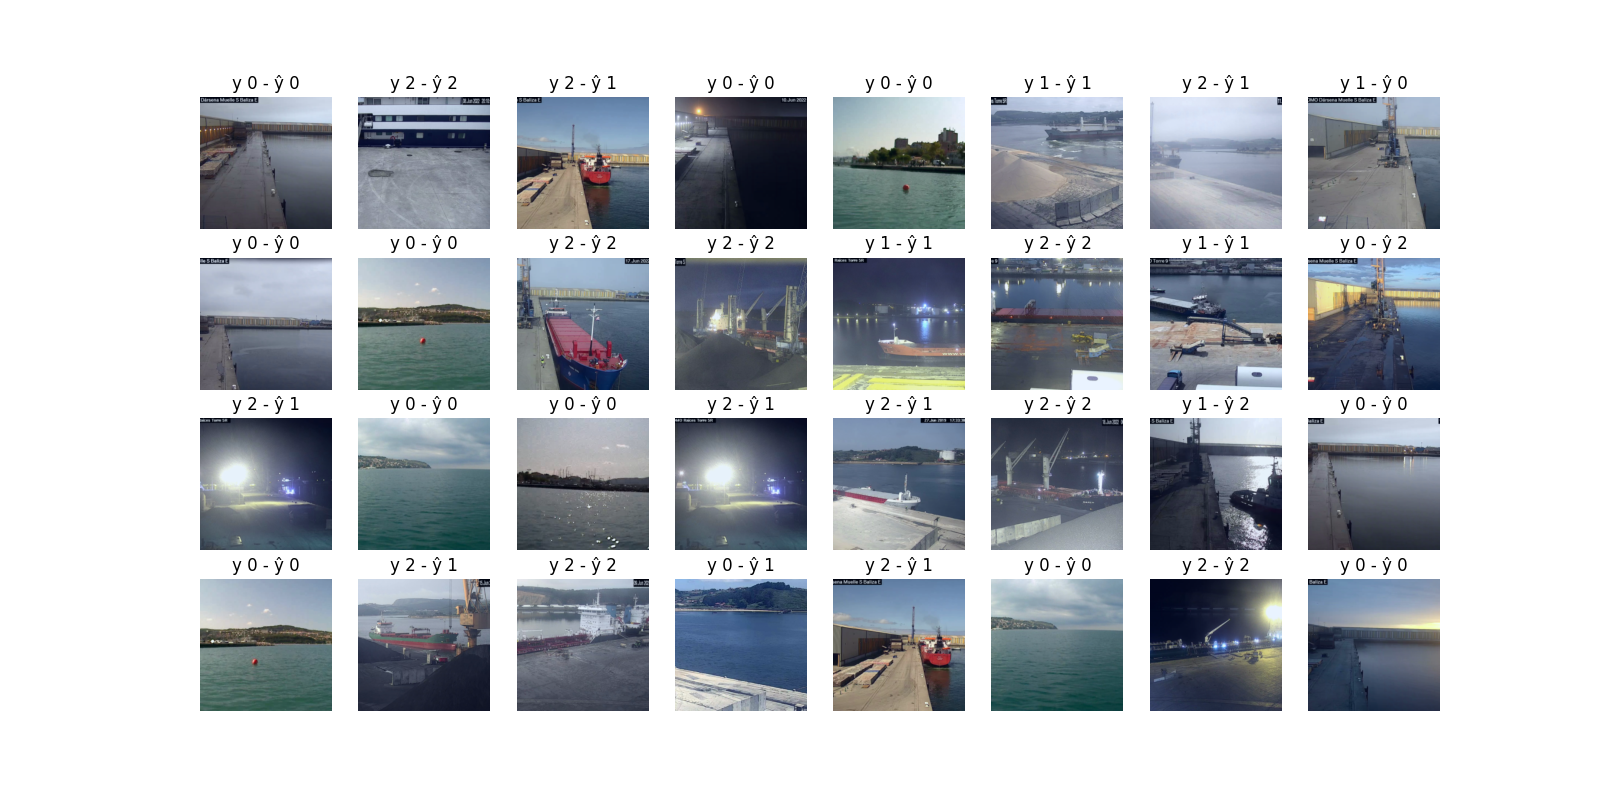
\includegraphics[width=\linewidth]{../ultimas_figuras/GRID__A_False_P_False_D_True_MLP_True_efficientnet_b4.png}
    \end{minipage}
\end{figure}
\subsubsection{Sen Aumento de datos e con Preentrenado}
\begin{figure}[H]
    \centering
    \begin{minipage}{0.55\textwidth}
        \centering
        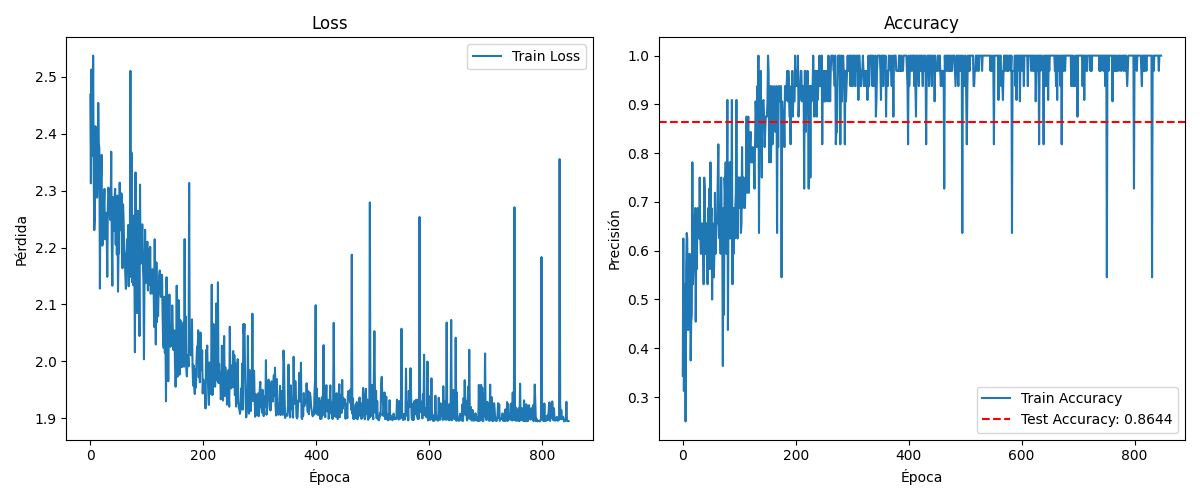
\includegraphics[width=\linewidth]{../ultimas_figuras/LOSS__A_False_P_True_D_True_MLP_True_efficientnet_b4.png}
    \end{minipage}
    \begin{minipage}{0.3\textwidth}
        \centering
        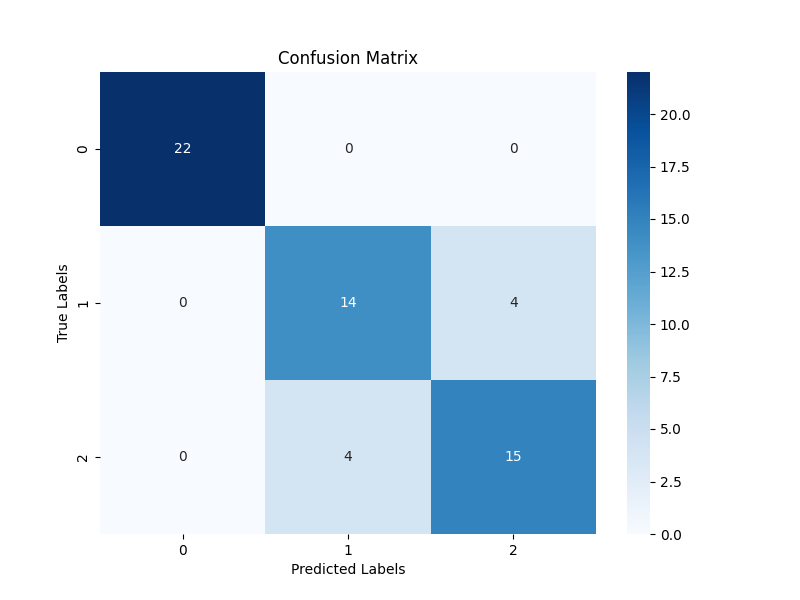
\includegraphics[width=\linewidth]{../ultimas_figuras/CM__A_False_P_True_D_True_MLP_True_efficientnet_b4.png}
    \end{minipage}
    \begin{minipage}{0.7\textwidth}
        \centering
        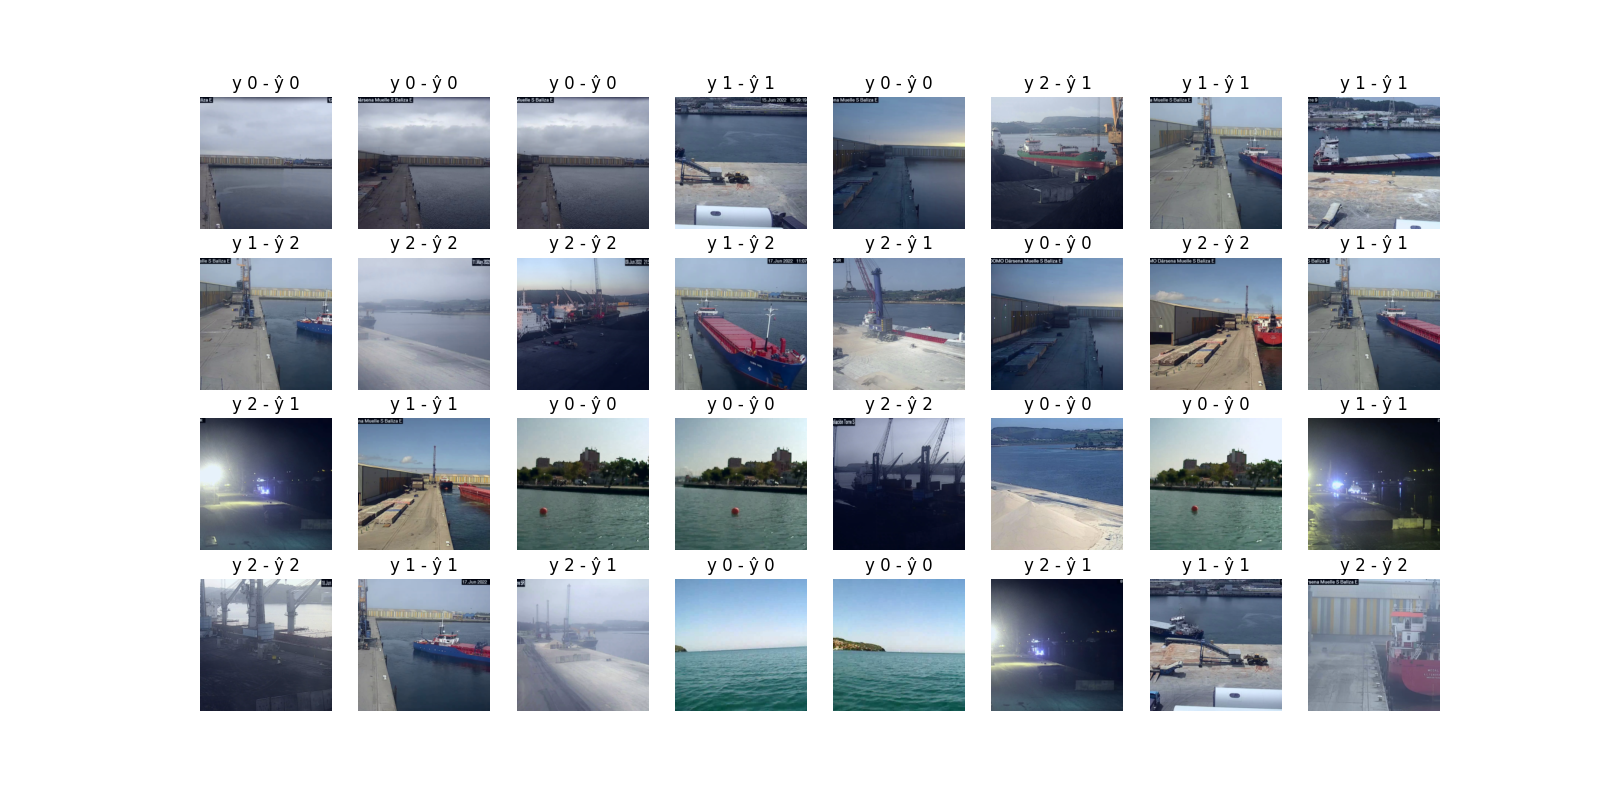
\includegraphics[width=\linewidth]{../ultimas_figuras/GRID__A_False_P_True_D_True_MLP_True_efficientnet_b4.png}
    \end{minipage}
\end{figure}
\subsubsection{Con Aumento de datos e sen Preentrenado}
\begin{figure}[H]
    \centering
    \begin{minipage}{0.55\textwidth}
        \centering
        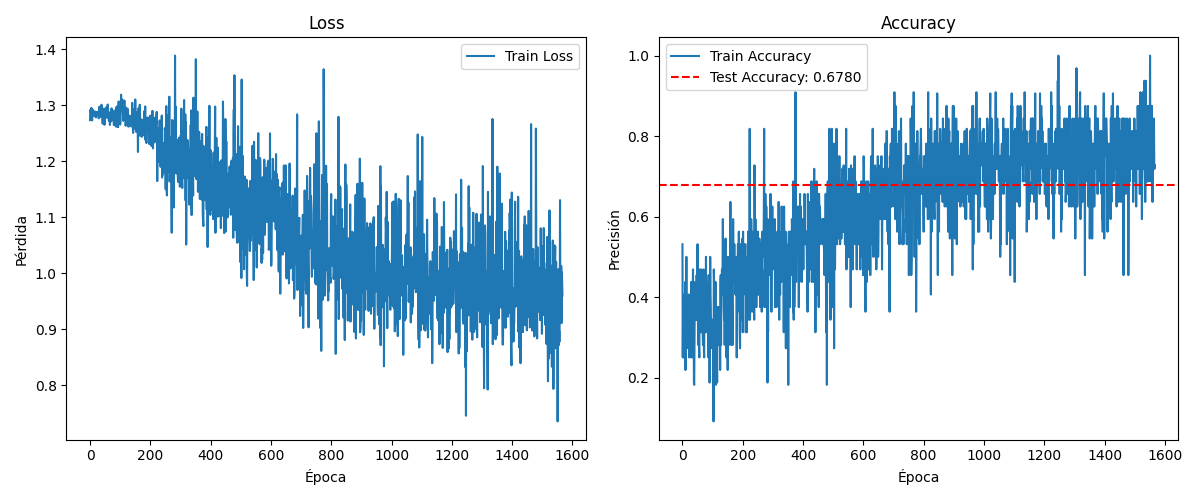
\includegraphics[width=\linewidth]{../ultimas_figuras/LOSS__A_True_P_False_D_True_MLP_True_efficientnet_b4.png}
    \end{minipage}
    \begin{minipage}{0.3\textwidth}
        \centering
        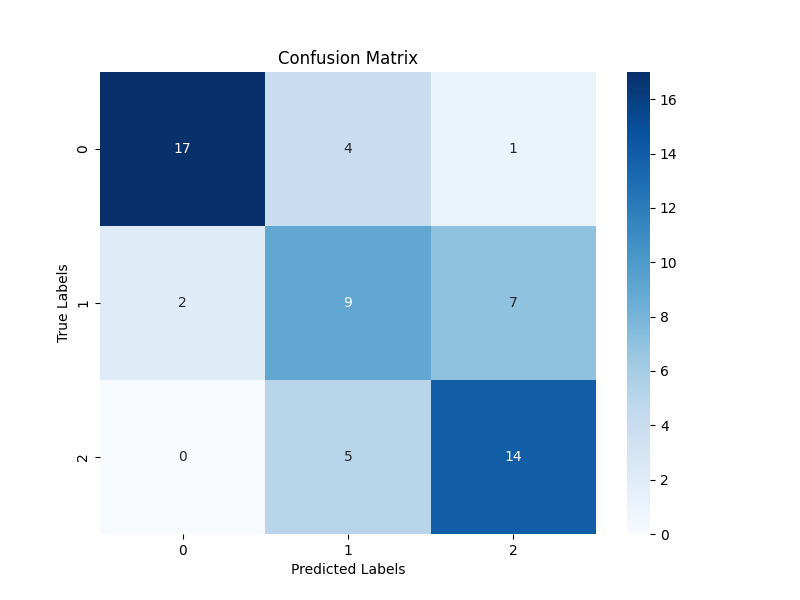
\includegraphics[width=\linewidth]{../ultimas_figuras/CM__A_True_P_False_D_True_MLP_True_efficientnet_b4.png}
    \end{minipage}
    \begin{minipage}{0.7\textwidth}
        \centering
        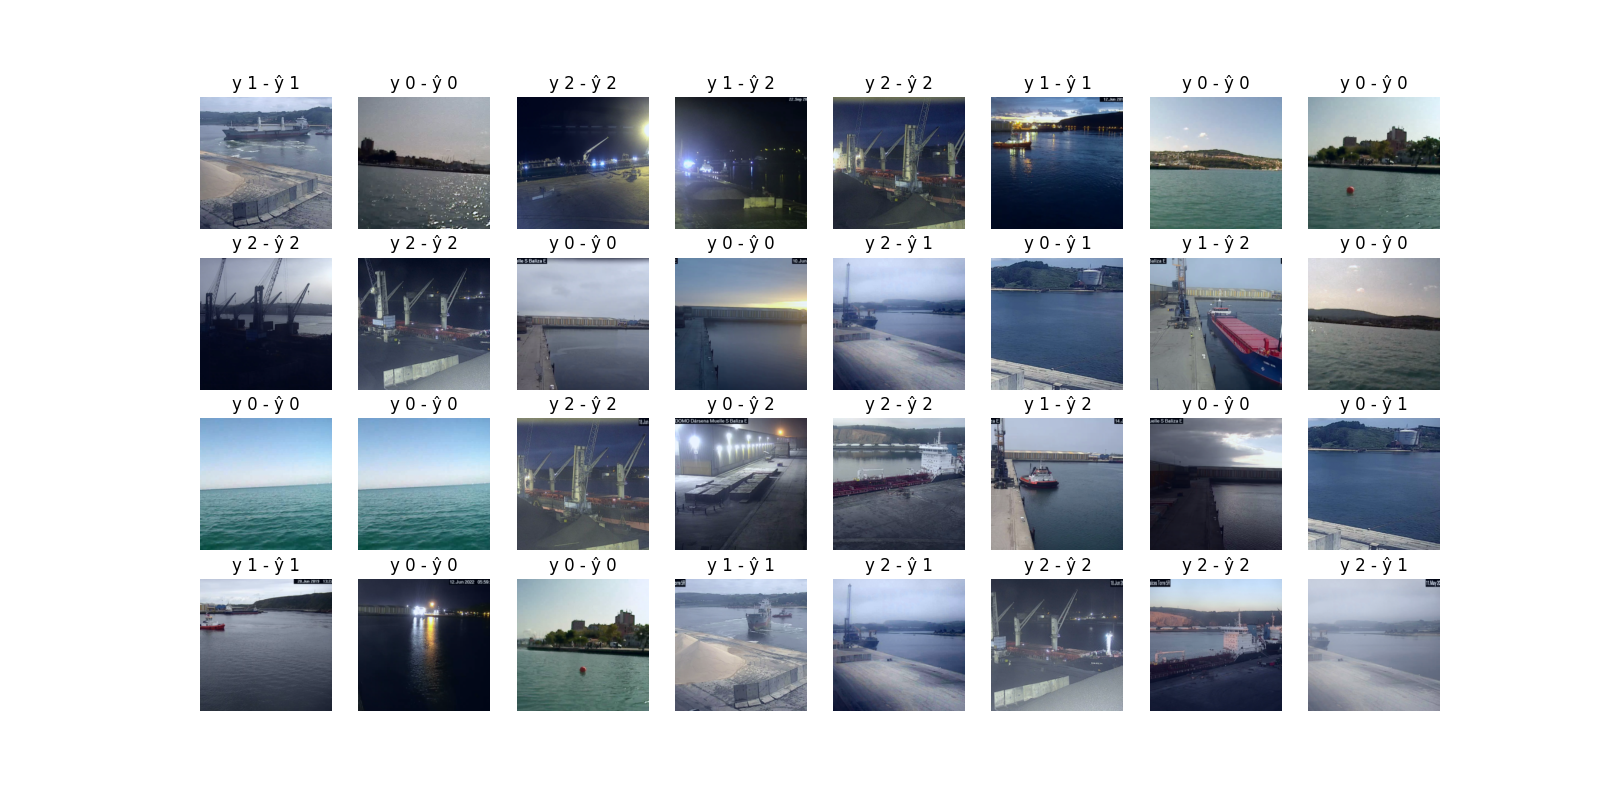
\includegraphics[width=\linewidth]{../ultimas_figuras/GRID__A_True_P_False_D_True_MLP_True_efficientnet_b4.png}
    \end{minipage}
\end{figure}
\subsubsection{Con Aumento de datos e con Preentrenado}
\begin{figure}[H]
    \centering
    \begin{minipage}{0.55\textwidth}
        \centering
        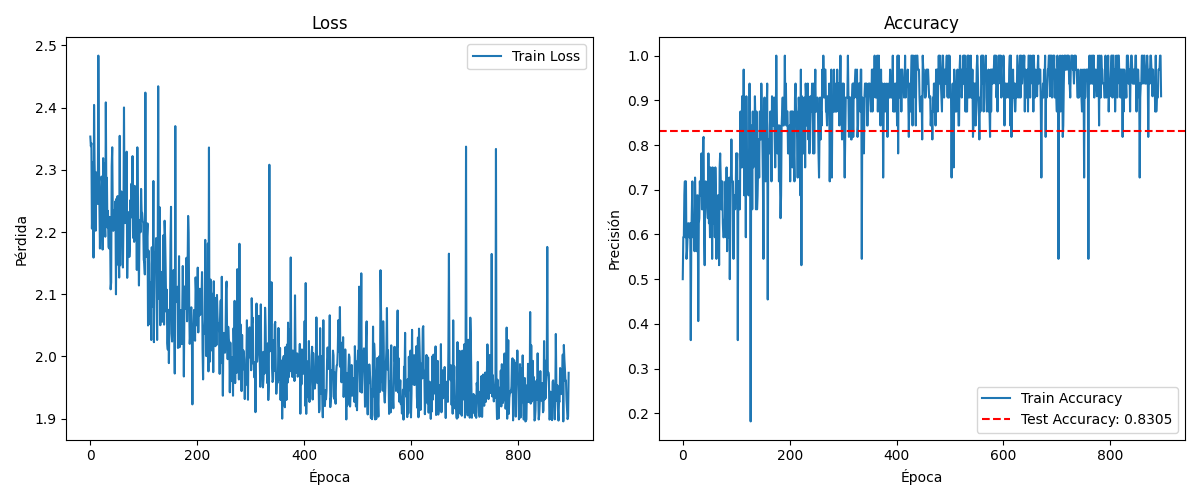
\includegraphics[width=\linewidth]{../ultimas_figuras/LOSS__A_True_P_True_D_True_MLP_True_efficientnet_b4.png}
    \end{minipage}
    \begin{minipage}{0.3\textwidth}
        \centering
        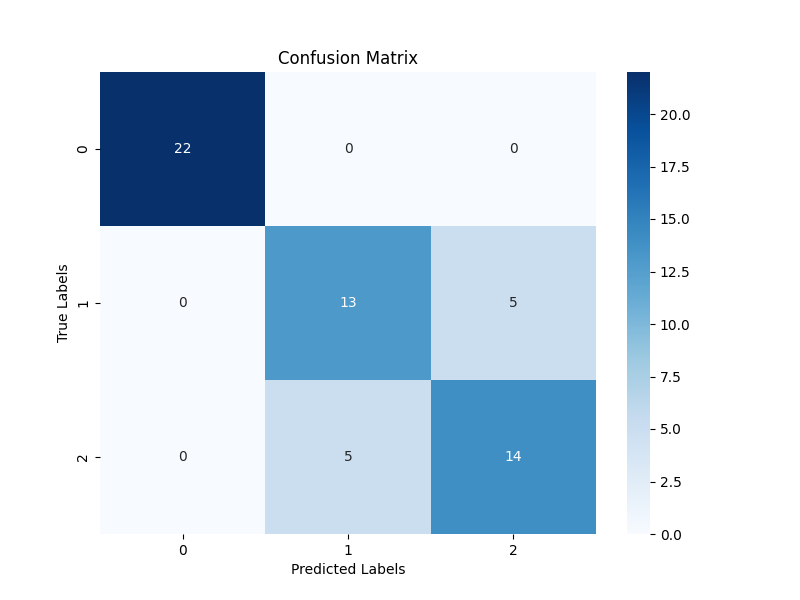
\includegraphics[width=\linewidth]{../ultimas_figuras/CM__A_True_P_True_D_True_MLP_True_efficientnet_b4.png}
    \end{minipage}
    \begin{minipage}{0.7\textwidth}
        \centering
        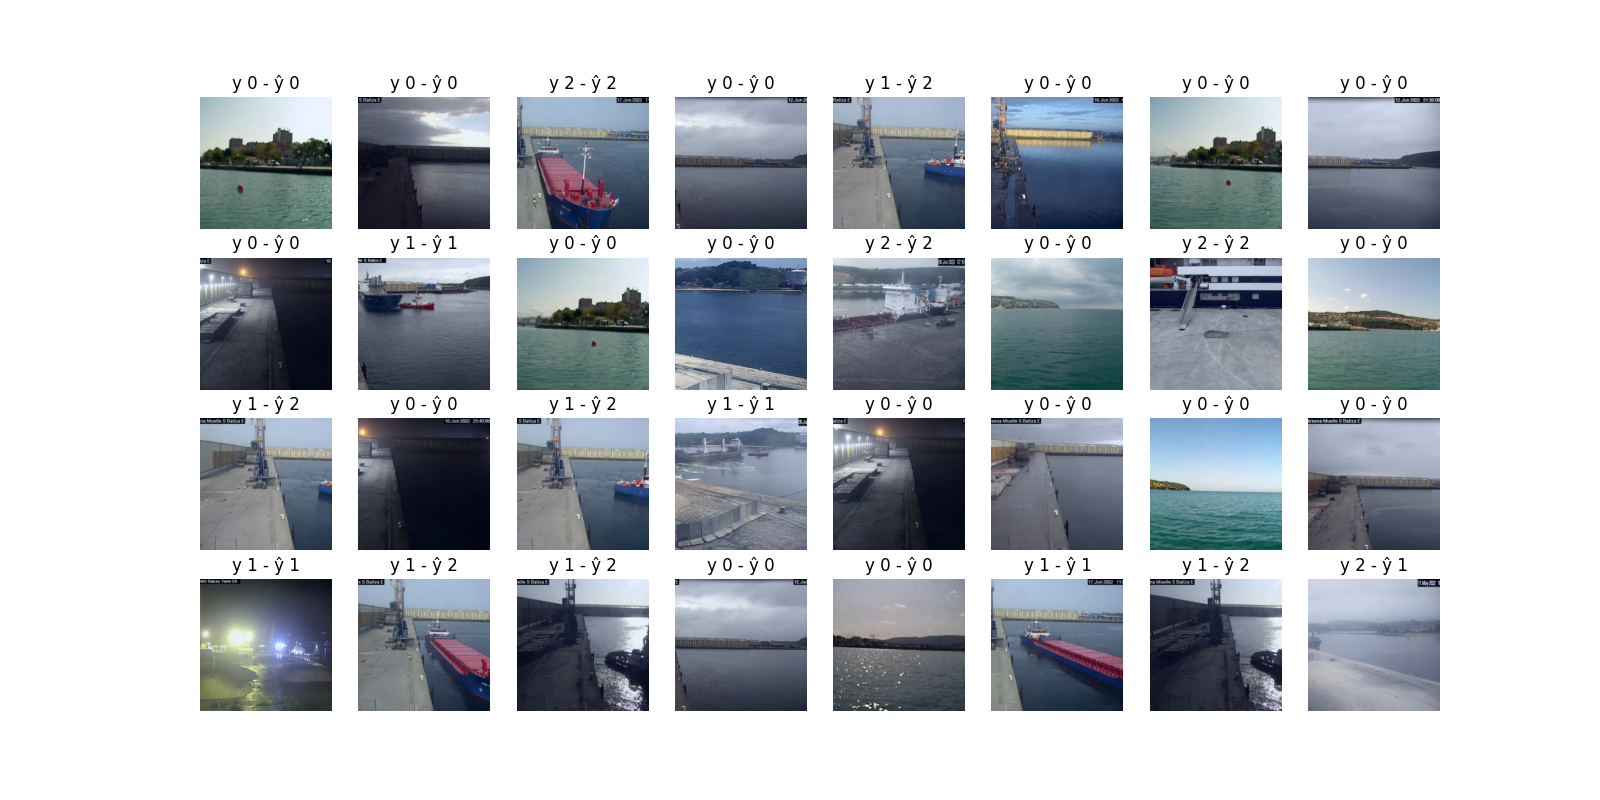
\includegraphics[width=\linewidth]{../ultimas_figuras/GRID__A_True_P_True_D_True_MLP_True_efficientnet_b4.png}
    \end{minipage}
\end{figure}

\newpage
\section{Apéndice B: como executar o noso código}

Para probar o primeiro e segundo exercicio con novas imaxes pode facerse algo así:

\begin{clibox}
\$ python main.py --load\_model   --model\_path ex1params --test\_images imagen.jpg imagen2.jpg imagen3.jpg --not\_train --mlp\_head

\$ python main.py --load\_model  --docked --model\_path ex2params --test\_images imagen.jpg imagen2.jpg imagen3.jpg --not\_train --mlp\_head


\end{clibox}


Donde o programa respondería con \footnote{As imaxes \texttt{imagen.jpg}, \texttt{imagen2.jpg} e \texttt{imagen3.jpg} poden atoparse na entrega e se examínanse, pode verse como efectivamente, a primeira é unha imaxen de barco atracado, a segunda e a mesma imaxen pero recortada (sen ruído a confianza da rede aumenta levemente) e a terceira é tamén un recorte da primeira pero esta vez do chan (consideramos oportuno que a Rede clasifique este tipo de imaxes como clase 0, é dicir, sabe que non hai un barco).}:

\begin{clibox}

Model loaded from ex2params

Testing individual images:

Image: imagen.jpg

Prediction: Ship (Docked)

Confidence: tensor([0.2157, 0.2130, 0.5713], device='mps:0')
%------------------------------

Image: imagen2.jpg

Prediction: Ship (Docked)

Confidence: tensor([0.2120, 0.2120, 0.5761], device='mps:0')
%------------------------------

Image: imagen3.jpg

Prediction: No Ship

Confidence: tensor([0.5737, 0.2129, 0.2134], device='mps:0')
\end{clibox}

Ou adicionalmente, no \texttt{pruebas.ipynb}:

\begin{figure}[H]
	\centering
	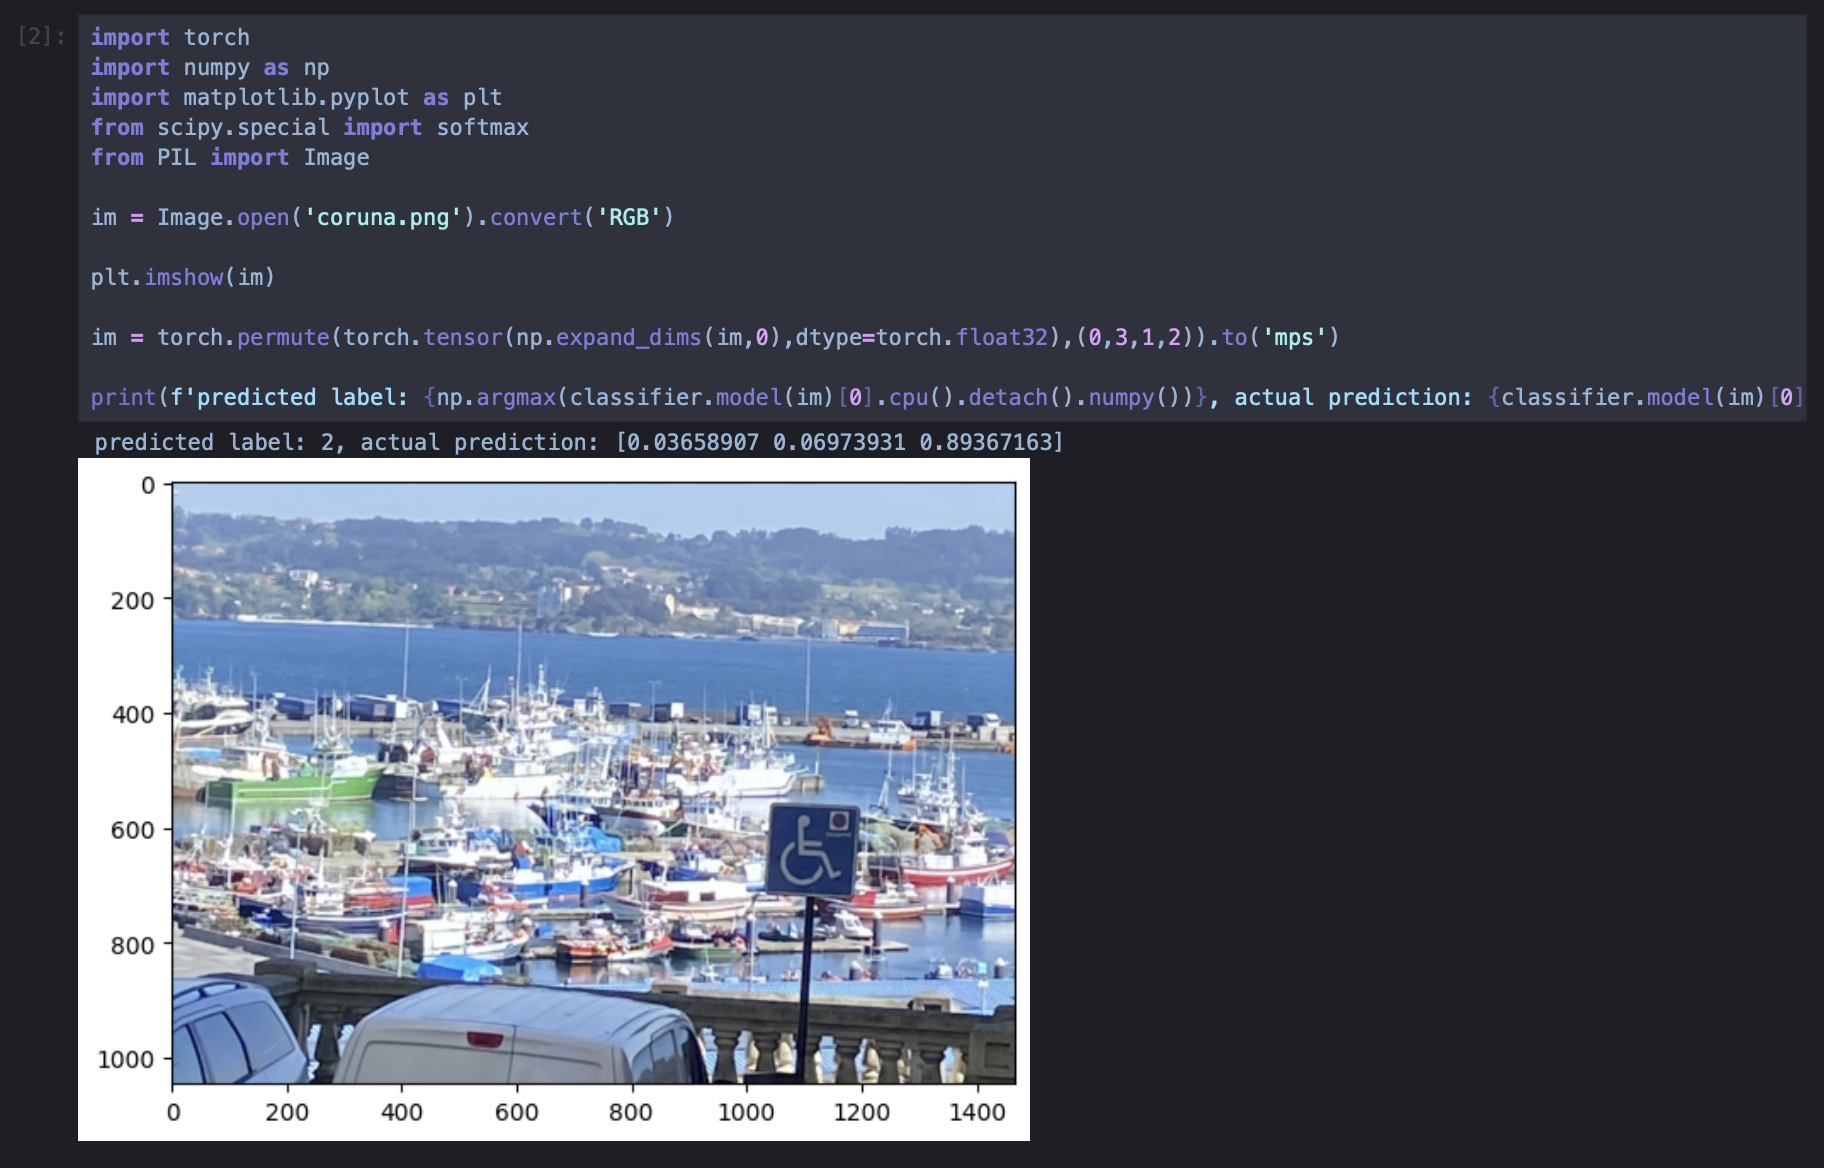
\includegraphics[width=0.8\linewidth]{ejecucion.png}
\end{figure}

Como nota final podemos decir que a foto superior sacouse no porto de Os Castros en A Coruña e o modelo predice que é unha foto con \emph{barco atracado}, e faino ainda que tanto os barcos como o peirao sexan distintos do que estivo acostumado a ver no adestramento.

\newpage

\bibliographystyle{plain}
\bibliography{referencias}



\end{document}

